\chapter{Results}
\label{ch:results}

\section{Overview}
This chapter presents (i) baseline performance of the ETA model across normal and rain scenarios, (ii) adaptation via incremental retraining after detected drift, and (iii) a head-to-head comparison of the initial vs.\ retrained models on the same post-swap evaluation window.
We conclude with a concise demonstration of the operational platform, meaning the dashboards, notifications, and reports.

\section{Notation and Setup}

Let $t \in [0, 72{,}000]$ denote simulation time in seconds. We define the following time windows:
\[
    \begin{aligned}
        W_{\text{test}} &= [0, 36{,}000),\\
        t_{\text{rain}} &= 36{,}000,\\
        W_{\text{rain}} &= [36{,}000, 72{,}000],\\
        t_{\text{drift}} &= 38{,}400,\\
        W_{\text{retrain}} &= [38{,}400, 42{,}000],\\
        t_{\text{swap}} &= 43{,}200,\\
        W_{\text{eval}} &= [43{,}200, 72{,}000].
    \end{aligned}
\]

\section{Models and Metrics}
\paragraph{Models.} We compare two models:

\begin{itemize}
    \item \textbf{Initial model} $M_0$: trained on 10~hours of normal data (initial training set size $53{,}229$).
    \item \textbf{Retrained model} $M_1$: incrementally fine-tuned on $W_{\text{retrain}}$ using 1 hour of samples or $6{,}755$ samples ($\approx 12.69\%$ of the initial training volume) and deployed at $t_{\text{swap}}=43{,}200$.
\end{itemize}

\paragraph{Metrics.} We use Mean Absolute Error (MAE) and Mean Absolute Percentage Error (MAPE) to evaluate the performance of the models:
\[
    \mathrm{MAE} = \frac{1}{n}\sum_{i=1}^{n} \bigl| y_i - \hat{y}_i \bigr|,
    \qquad
    \mathrm{MAPE} = \frac{100}{n}\sum_{i=1}^{n} \left| \frac{y_i - \hat{y}_i}{y_i} \right|\%.
\]
For relative improvements from model $A$ to $B$ we use
\[
    \Delta_{\%}(A \!\rightarrow\! B) = 100 \times \frac{A - B}{A}\, ,
\]
and we denote absolute differences in percentage points as ``pp''.

\section{Baseline Model Performance}

Table~\ref{tab:baseline} summarizes the performance of the initial model $M_0$ on the first day (normal conditions) and on the second day (rain conditions), before any adaptation.

\begin{table}[h]
    \centering
    \caption{Baseline results for $M_0$ (no adaptation), by scenario.}
    \label{tab:baseline}
    \begin{tabular}{lcc}
        \toprule
        Scenario / Window & MAE & MAPE \\
        \midrule
        First day $W_{\text{test}}$ & \textbf{30.36} & \textbf{13.20}\% \\
        Second day $W_{\text{rain}}$ & \textbf{56.93} & \textbf{19.02}\% \\
        \bottomrule
    \end{tabular}
\end{table}

Moving from normal to rain nearly doubles MAE (from 30.36 to 56.93) and raises MAPE from 13.20\% to 19.02\%, indicating a substantial scenario shift, a concept drift.

The evolution of the baseline model errors over time can be seen in the following \autoref{fig:baseline-errors}:

\begin{figure}[h]
    \centering
    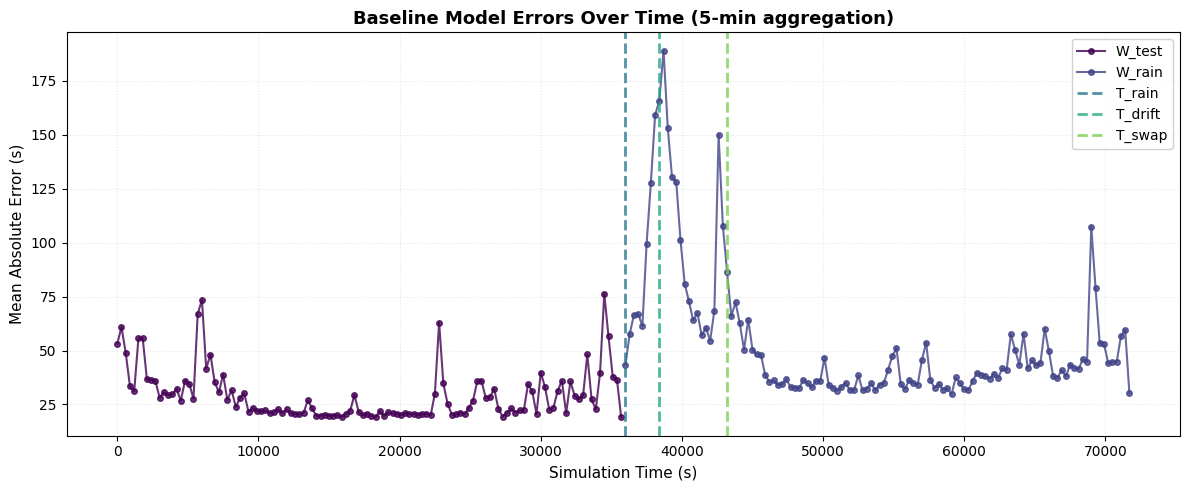
\includegraphics[width=\textwidth]{figures/baseline-errors.png}
    \caption{Baseline Model Errors Over Time.}
    \label{fig:baseline-errors}
\end{figure}

\section{Retrained Model: Training Window and Rationale}

A drift event is detected at $t_{\text{drift}}=38{,}400$ by the platform's drift detectors, running for this specific model.
To adapt, the platform fine-tunes $M_0$ on the first hour of post-drift rain data, i.e., $W_{\text{retrain}}=[38{,}400, 42{,}000]$ (6\,755 samples, $\approx12.69\%$ of the initial training volume).
The updated model $M_1$ is then hot-swapped at $t_{\text{swap}}=43{,}200$.

This choice targets the specific post-drift distribution and with only an hour of data and a quick retraining time, it allows for a seamless adaptation, producing an adapted model while the simulation continues.
We evaluate the effect of this adaptation on a clean hold-out: the remainder of the rain scenario after the recorded swap.

\section{Post-Swap Evaluation on an Identical Window}

To ensure a fair, apples-to-apples comparison, we evaluate both the non-adapted baseline ($M_0$) and the retrained model ($M_1$) on the \emph{same} post-swap window $W_{\text{eval}}=[43{,}200, 72{,}000]$.

\begin{table}[h]
    \centering
    \caption{Head-to-head results on the post-swap window $W_{\text{eval}}=[43{,}200, 72{,}000]$.}
    \label{tab:postswap}
    \begin{tabular}{lcc}
        \toprule
        Model (Window) & MAE & MAPE \\
        \midrule
        $M_0$ (initial; $W_{\text{eval}}$) & \textbf{43.27} & \textbf{16.89}\% \\
        $M_1$ (retrained; $W_{\text{eval}}$) & \textbf{32.27} & \textbf{14.55}\% \\
        \midrule
        Absolute difference & \textbf{11.00}~s MAE & \textbf{2.34}~pp MAPE \\
        Relative change $\Delta_{\%}$ & \textbf{25.42}\% $\downarrow$ & \textbf{13.85}\% $\downarrow$ \\
        \bottomrule
    \end{tabular}
\end{table}

The retrained model reduces MAE by 11.00~s (25.42\%) and MAPE by 2.34~pp (13.85\%) versus the baseline on the post-swap window, evidencing effective adaptation to rain.

The post-swap comparison of the baseline and retrained models can be seen in the following \autoref{fig:postswap-comparison}:

\begin{figure}[h]
    \centering
    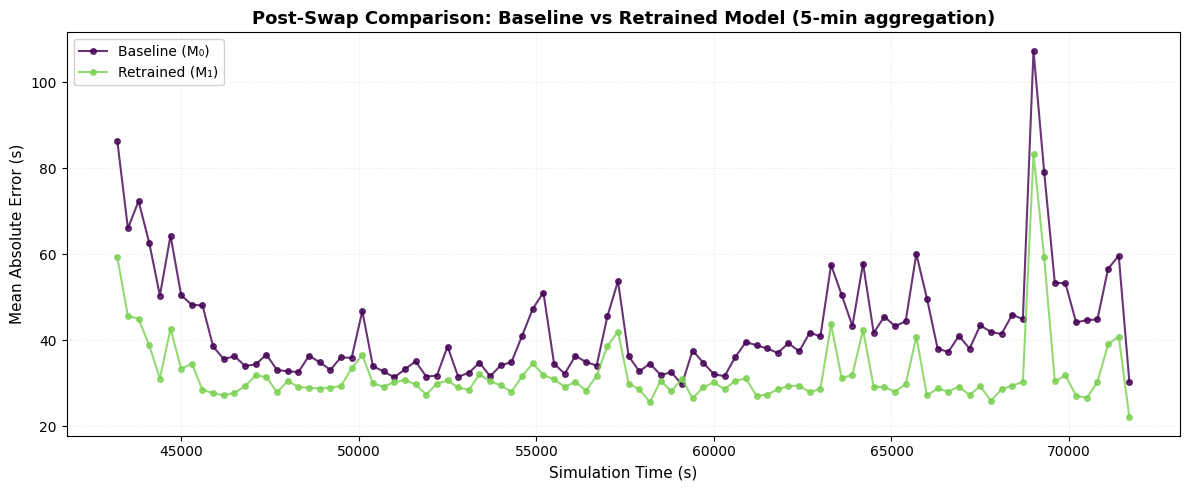
\includegraphics[width=\textwidth]{figures/postswap-comparison.png}
    \caption{Post-Swap Comparison: Baseline vs Retrained Model.}
    \label{fig:postswap-comparison}
\end{figure}

\section{Takeaways}
\paragraph{Baseline drift impact.}
From normal to rain, MAE rises from 30.36 to 56.93 and MAPE from 13.20\% to 19.02\%, confirming a substantial distribution shift.

\paragraph{Adaptation effectiveness.}
On the identical post-swap window $W_{\text{eval}}$, $M_1$ improves over $M_0$ by \textbf{11.00~s MAE} (25.42\%) and \textbf{2.34~pp MAPE} (13.85\%).

\paragraph{Operational closure of the loop.}
The platform detects drift, fine-tunes on $W_{\text{retrain}}$, and hot-swaps at $t{=}43{,}200$, showcasing a successful and seamless adaptation process.

\section{Platform Demonstration}

Figures~\ref{fig:dashboard-start}--\ref{fig:dashboard-report} illustrate the end-to-end run from an operator's perspective.
Each step shows either the \emph{Admin Dashboard} or the \emph{User Interface} to connect system state with user-facing predictions.

\paragraph{Narrative highlights.}
\emph{Start} $\rightarrow$ \emph{Stable} establishes the nominal baseline.
During \emph{Drifted}, rain conditions are active, all models experience performance degradation and all tasks are flagged as drifted.
In \emph{Retraining}, only ETA has been retrained and swapped, so the User Interface shows a higher ETA prediction for the same route while fuel and stops remain at their pre-adaptation values.
Finally, in \emph{Retrained}, all tasks are adapted and calibrated, and the User Interface reflects consistent post-recovery predictions.
The \emph{Report} view closes the loop with the AI generated summary report of the simulation, after it has completed.

\begin{figure}[p]
    \centering
    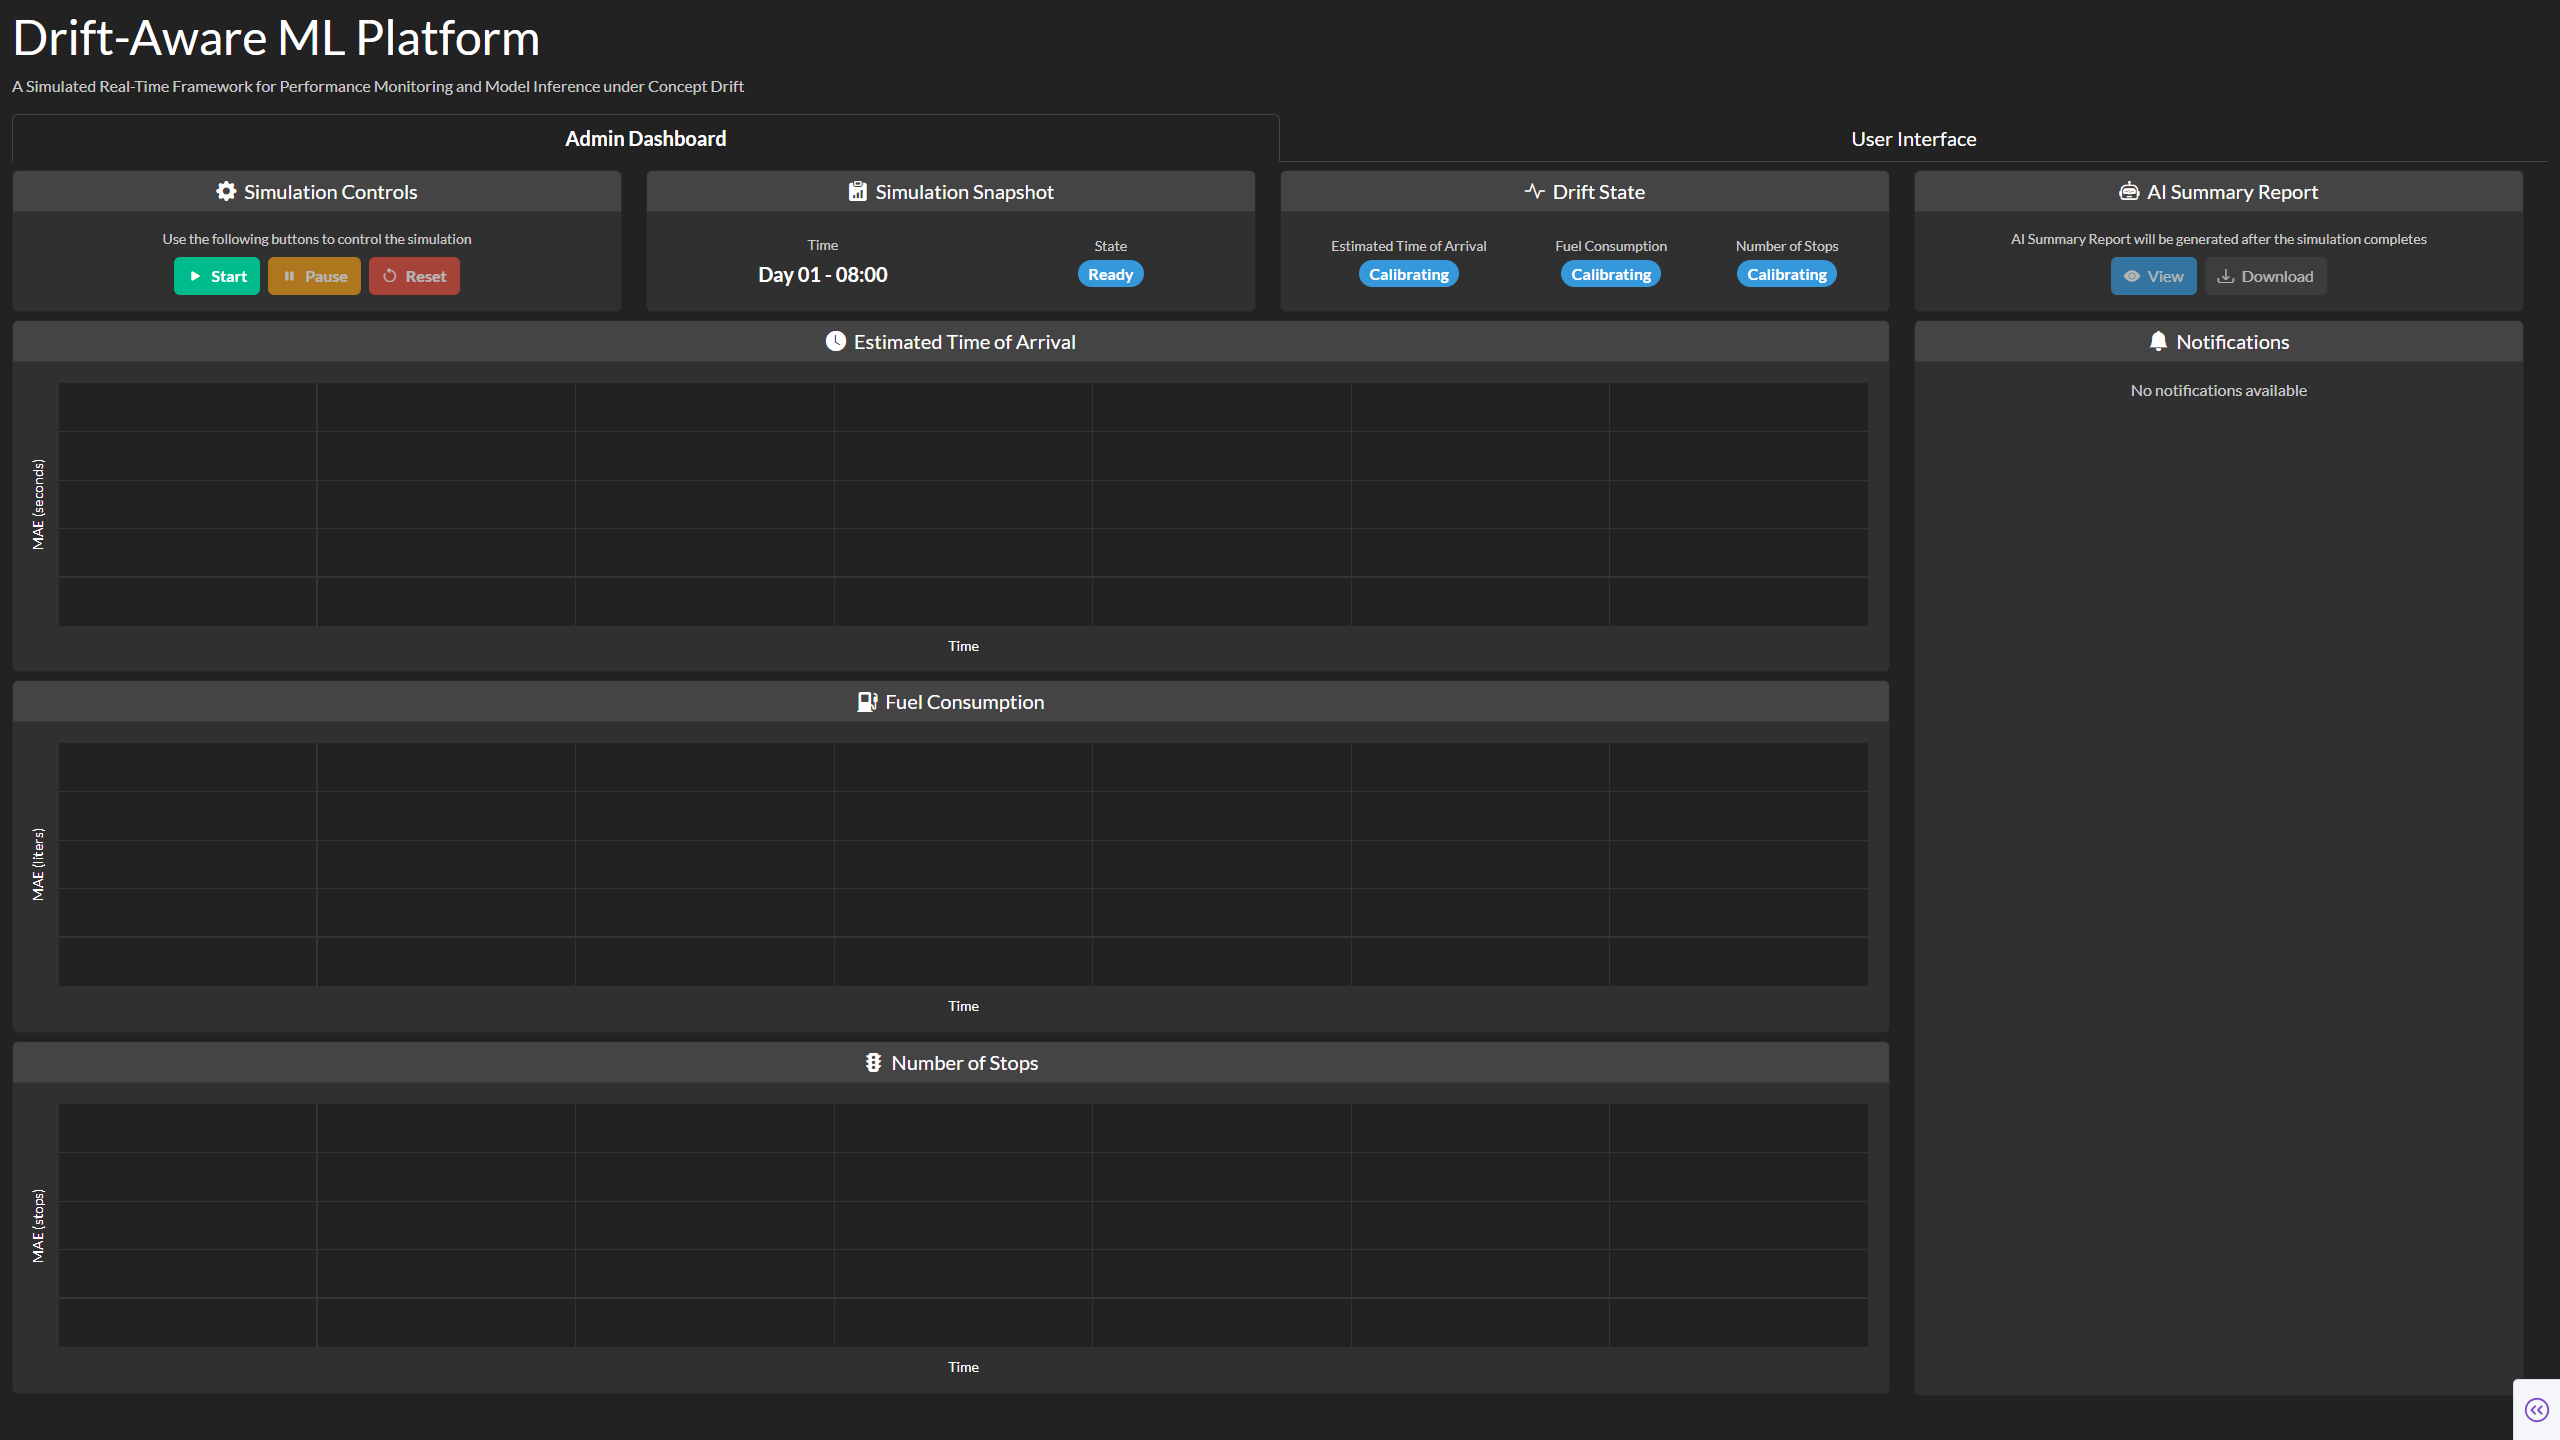
\includegraphics[width=\textwidth]{figures/dashboard-start.png}
    \caption{Admin dashboard --- \emph{Start}. Detectors calibrating, graphs empty, simulation not yet running.}
    \label{fig:dashboard-start}
\end{figure}

\begin{figure}[p]
    \centering
    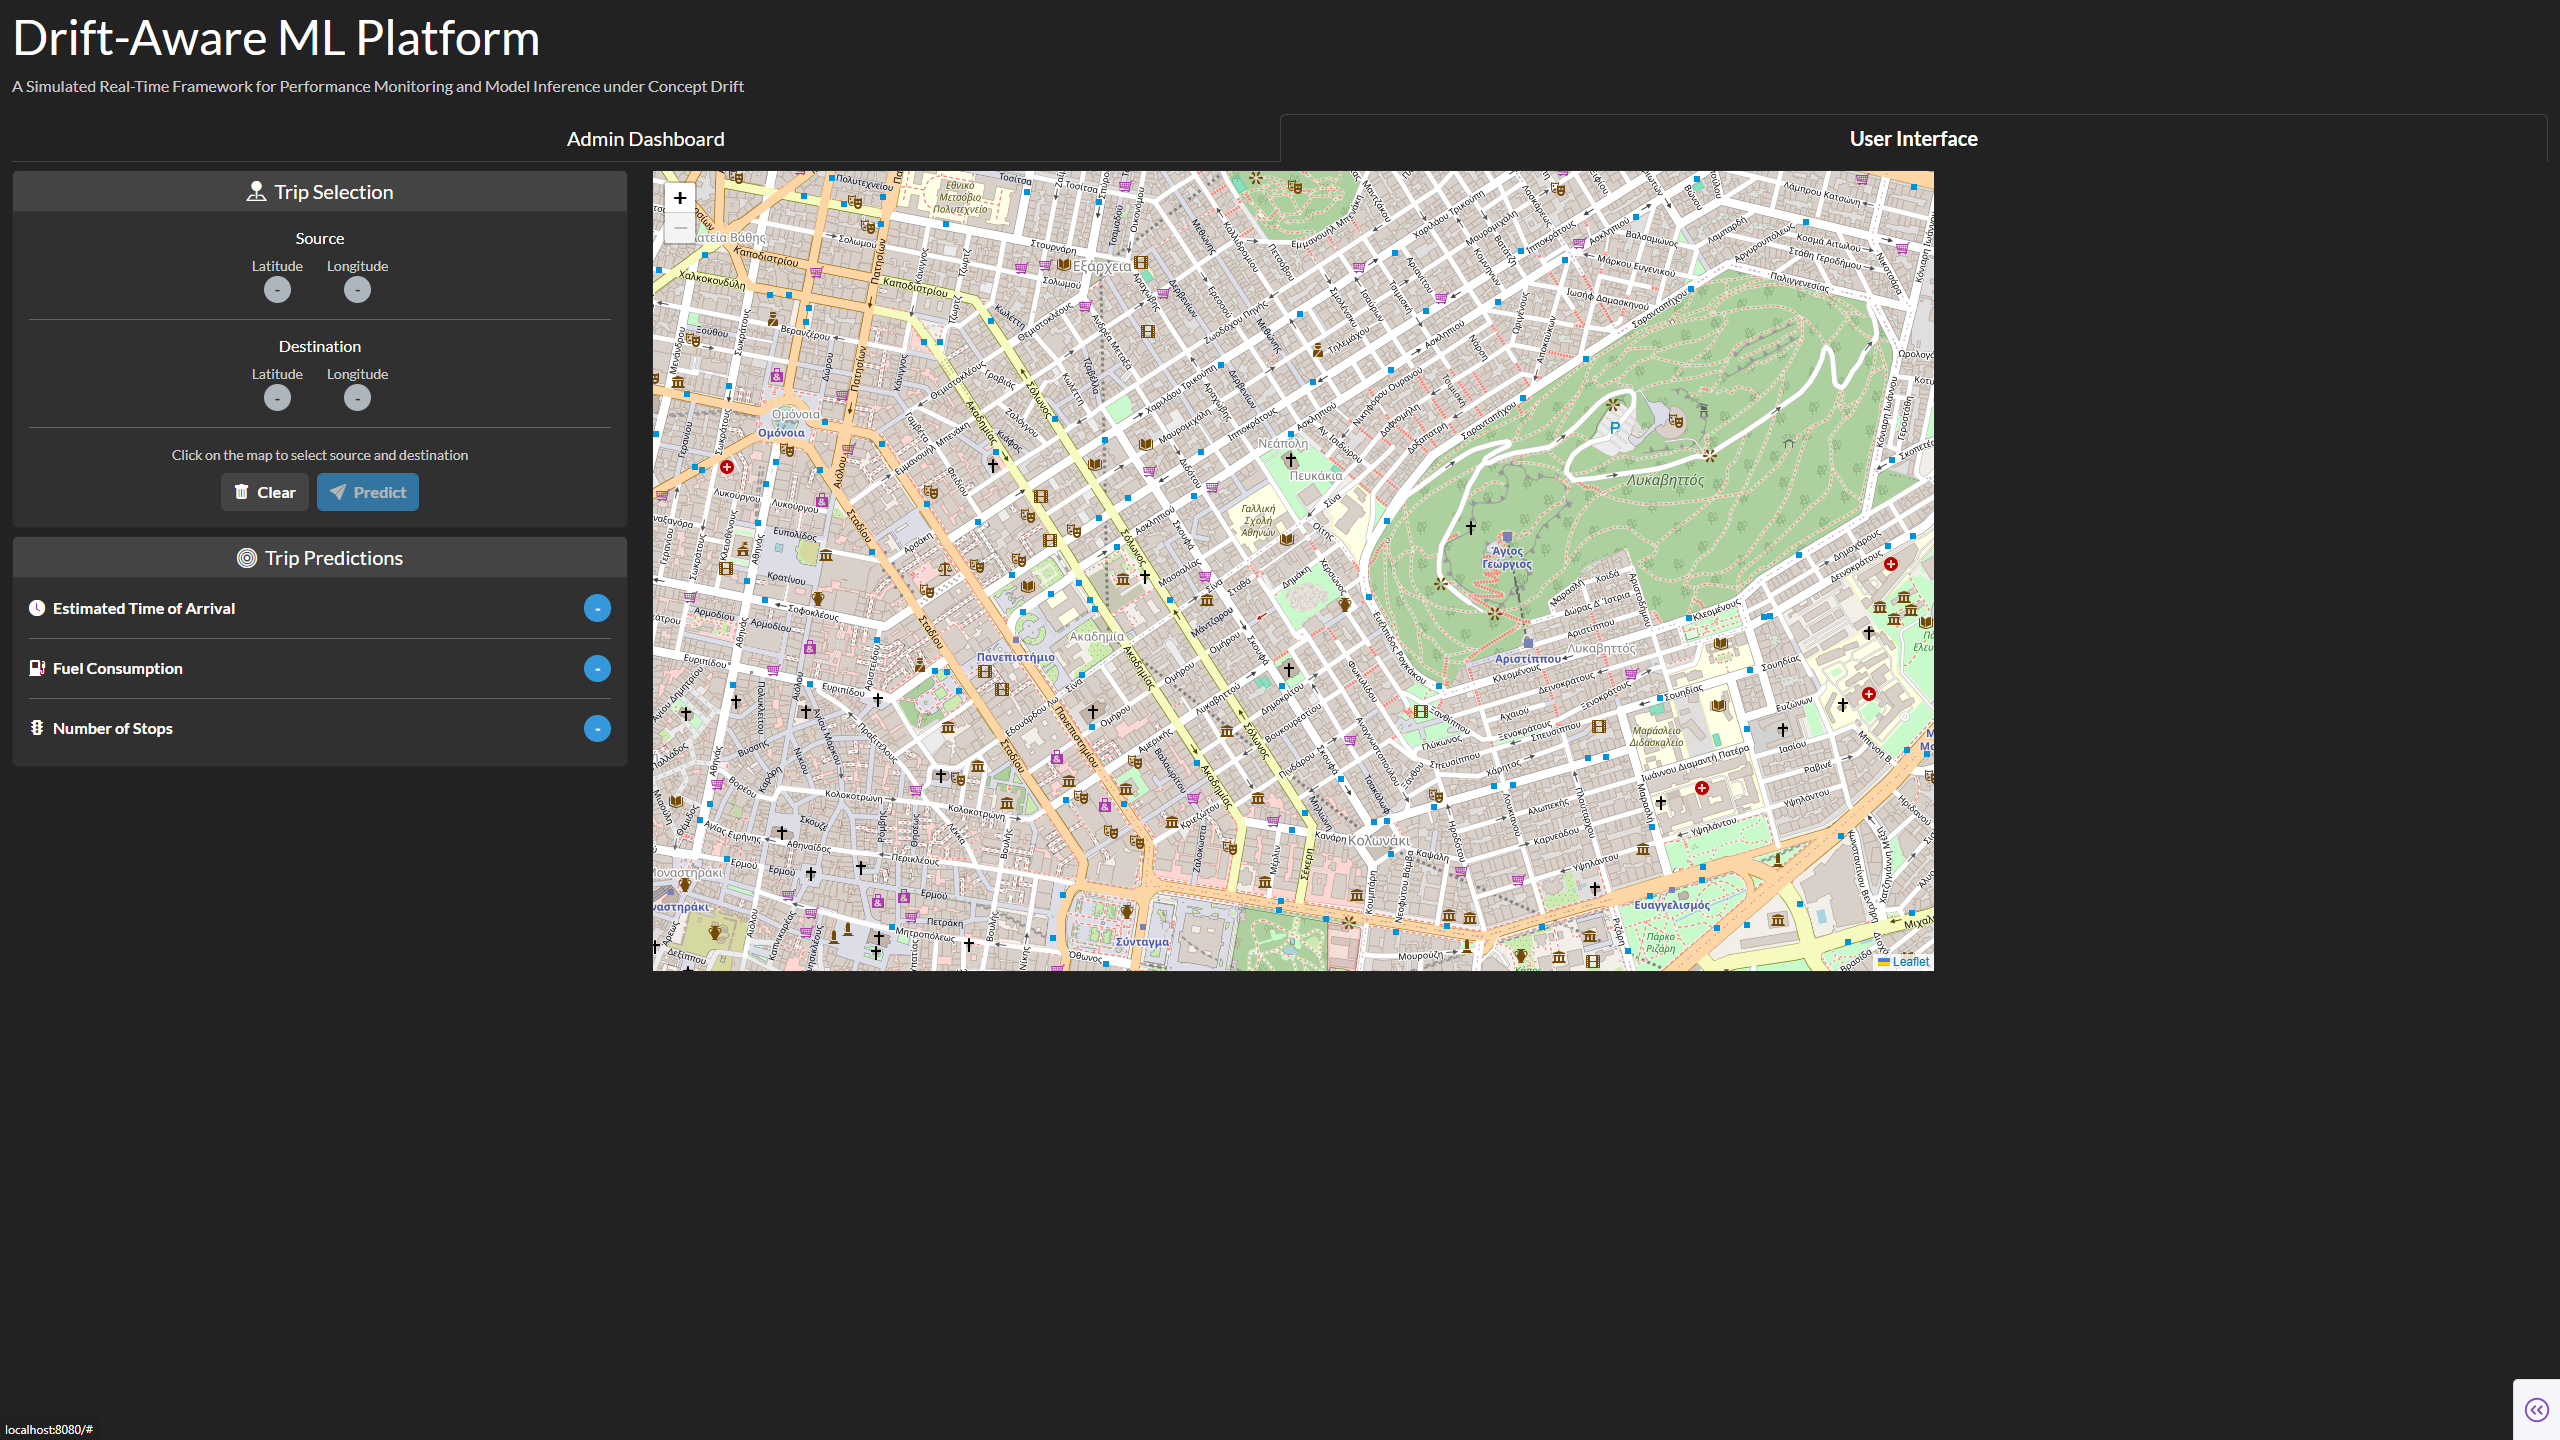
\includegraphics[width=\textwidth]{figures/ui-start.png}
    \caption{User interface --- \emph{Start}. No Source and Destination selected, prediction panels empty.}
    \label{fig:ui-start}
\end{figure}

\clearpage

\begin{figure}[p]
    \centering
    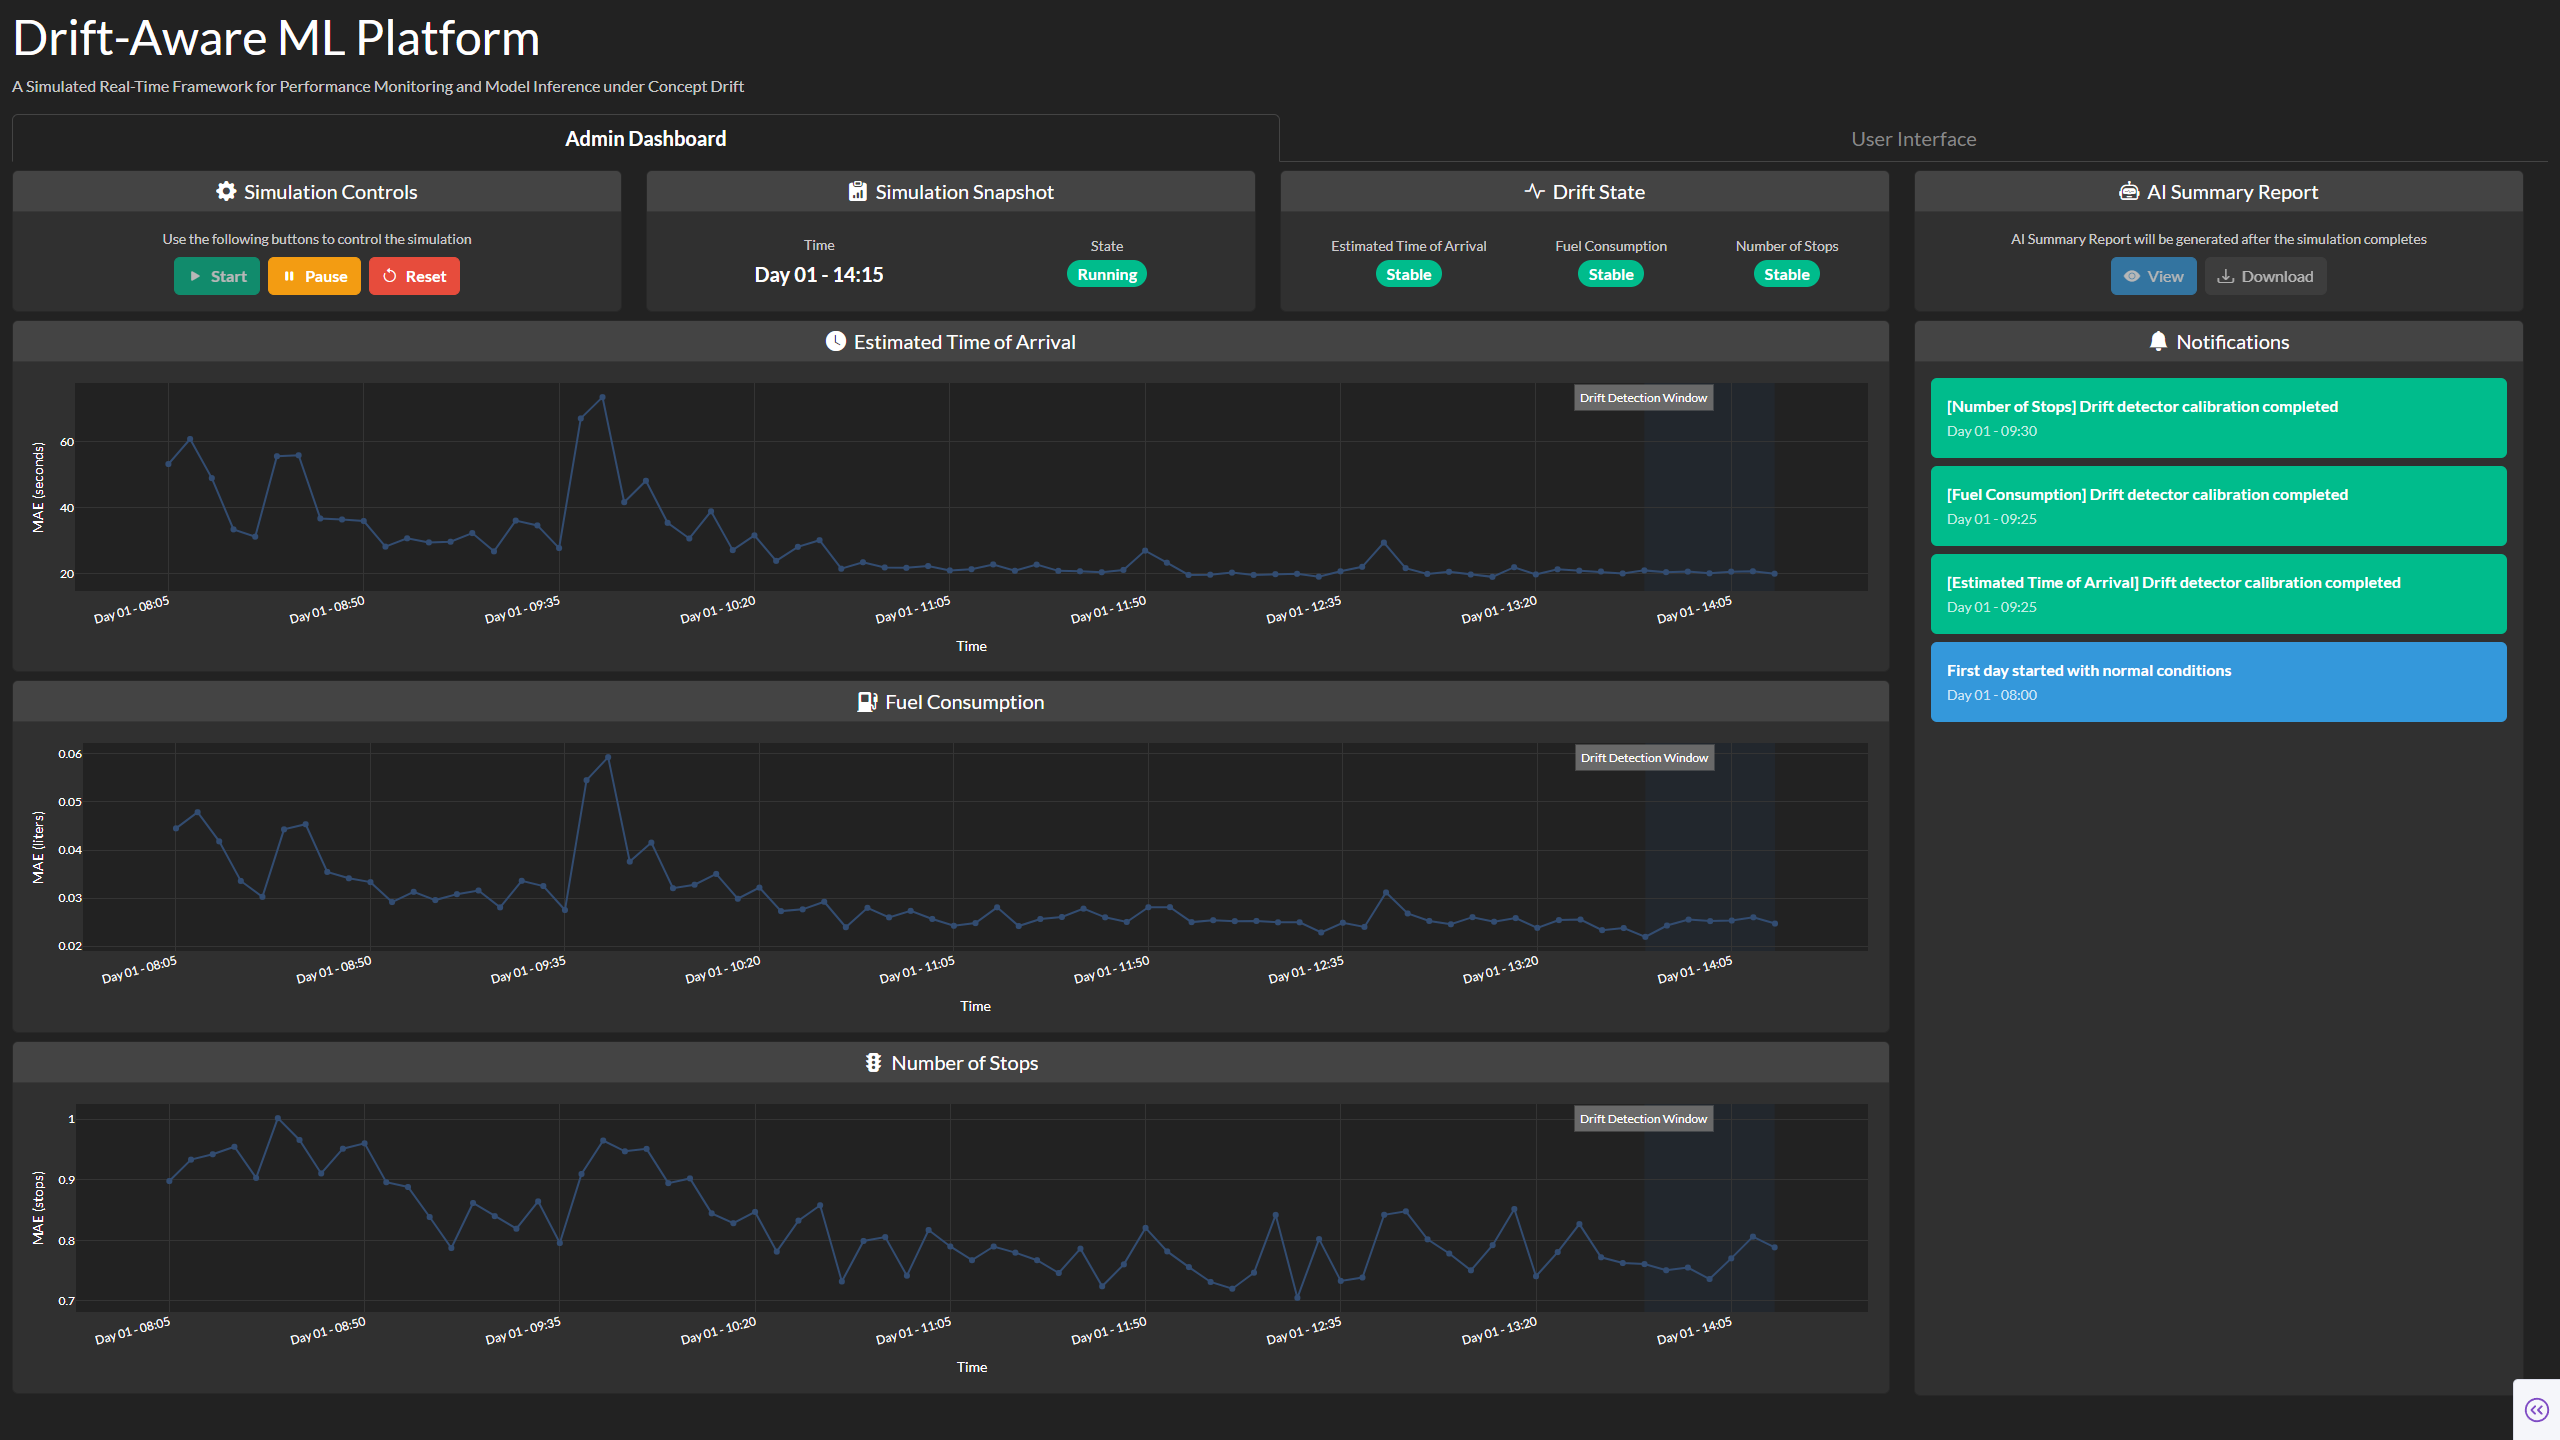
\includegraphics[width=\textwidth]{figures/dashboard-stable.png}
    \caption{Admin dashboard --- \emph{Stable}. Models stable under normal conditions, detectors calibrated.}
    \label{fig:dashboard-stable}
\end{figure}

\begin{figure}[p]
    \centering
    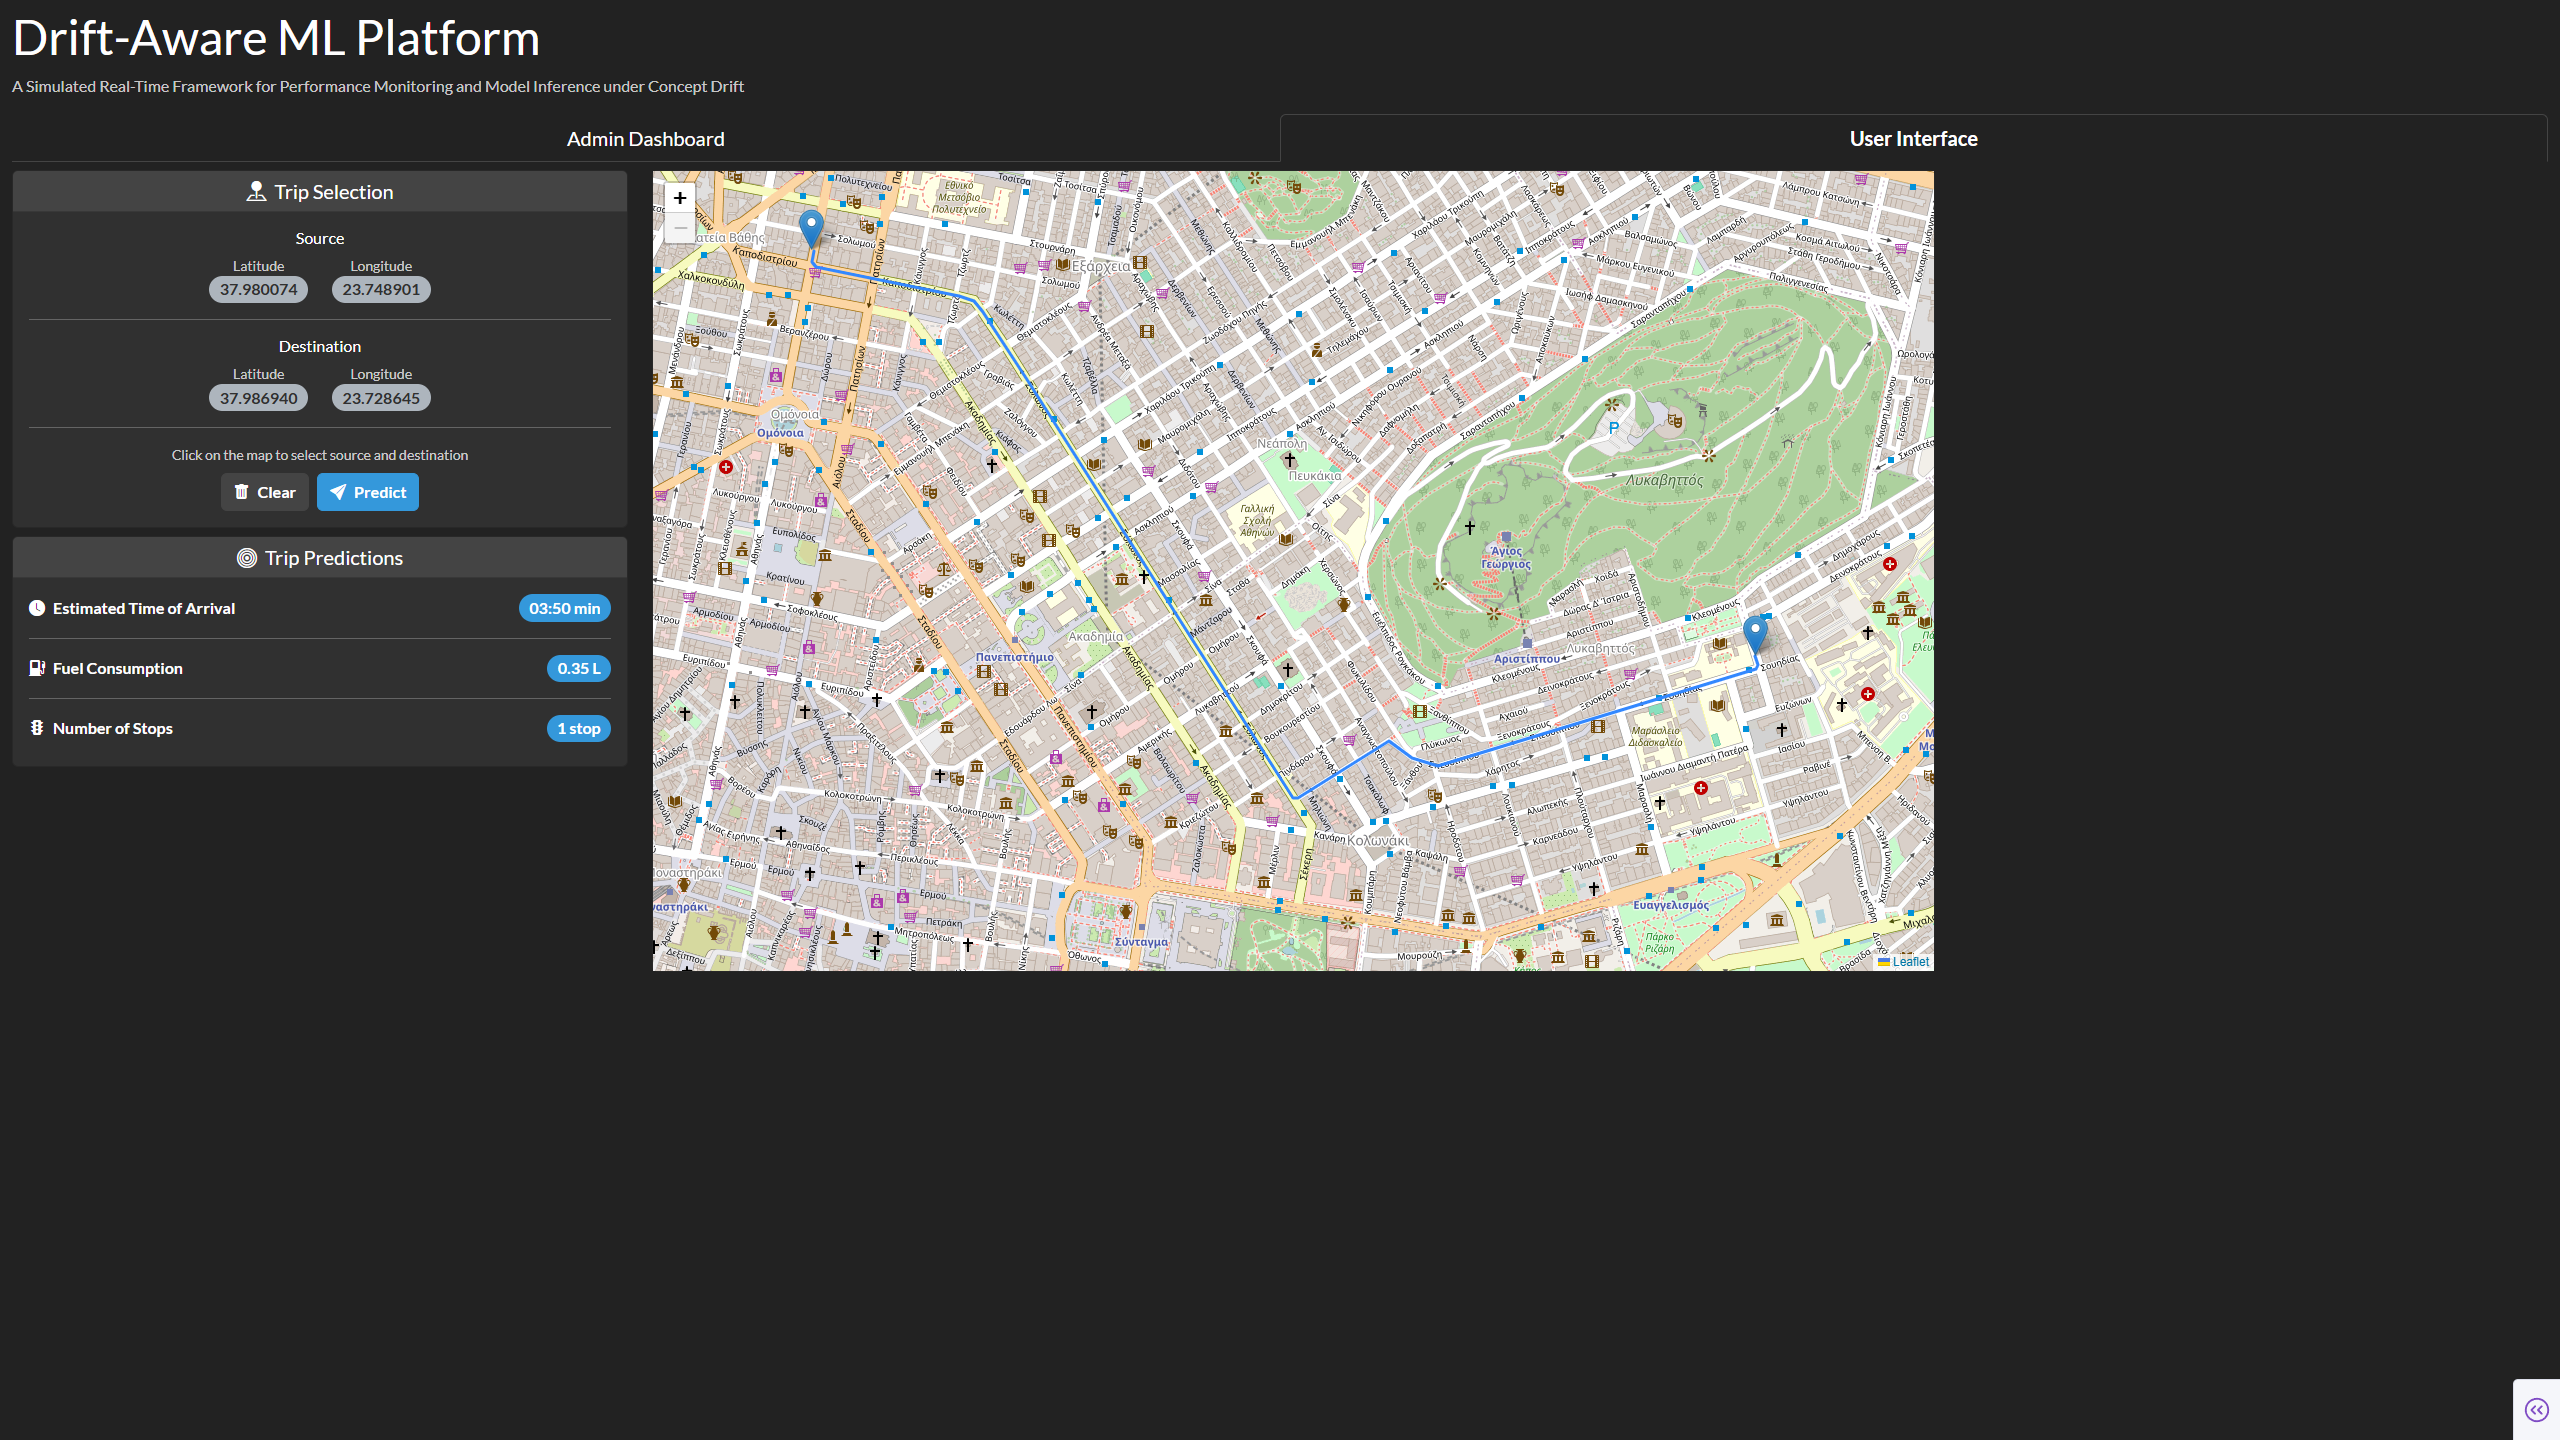
\includegraphics[width=\textwidth]{figures/ui-stable.png}
    \caption{User interface --- \emph{Stable}. Example route with baseline predictions: \texttt{03:50 min}, \texttt{0.35 L}, \texttt{1 stop}.}
    \label{fig:ui-stable}
\end{figure}

\clearpage

\begin{figure}[p]
    \centering
    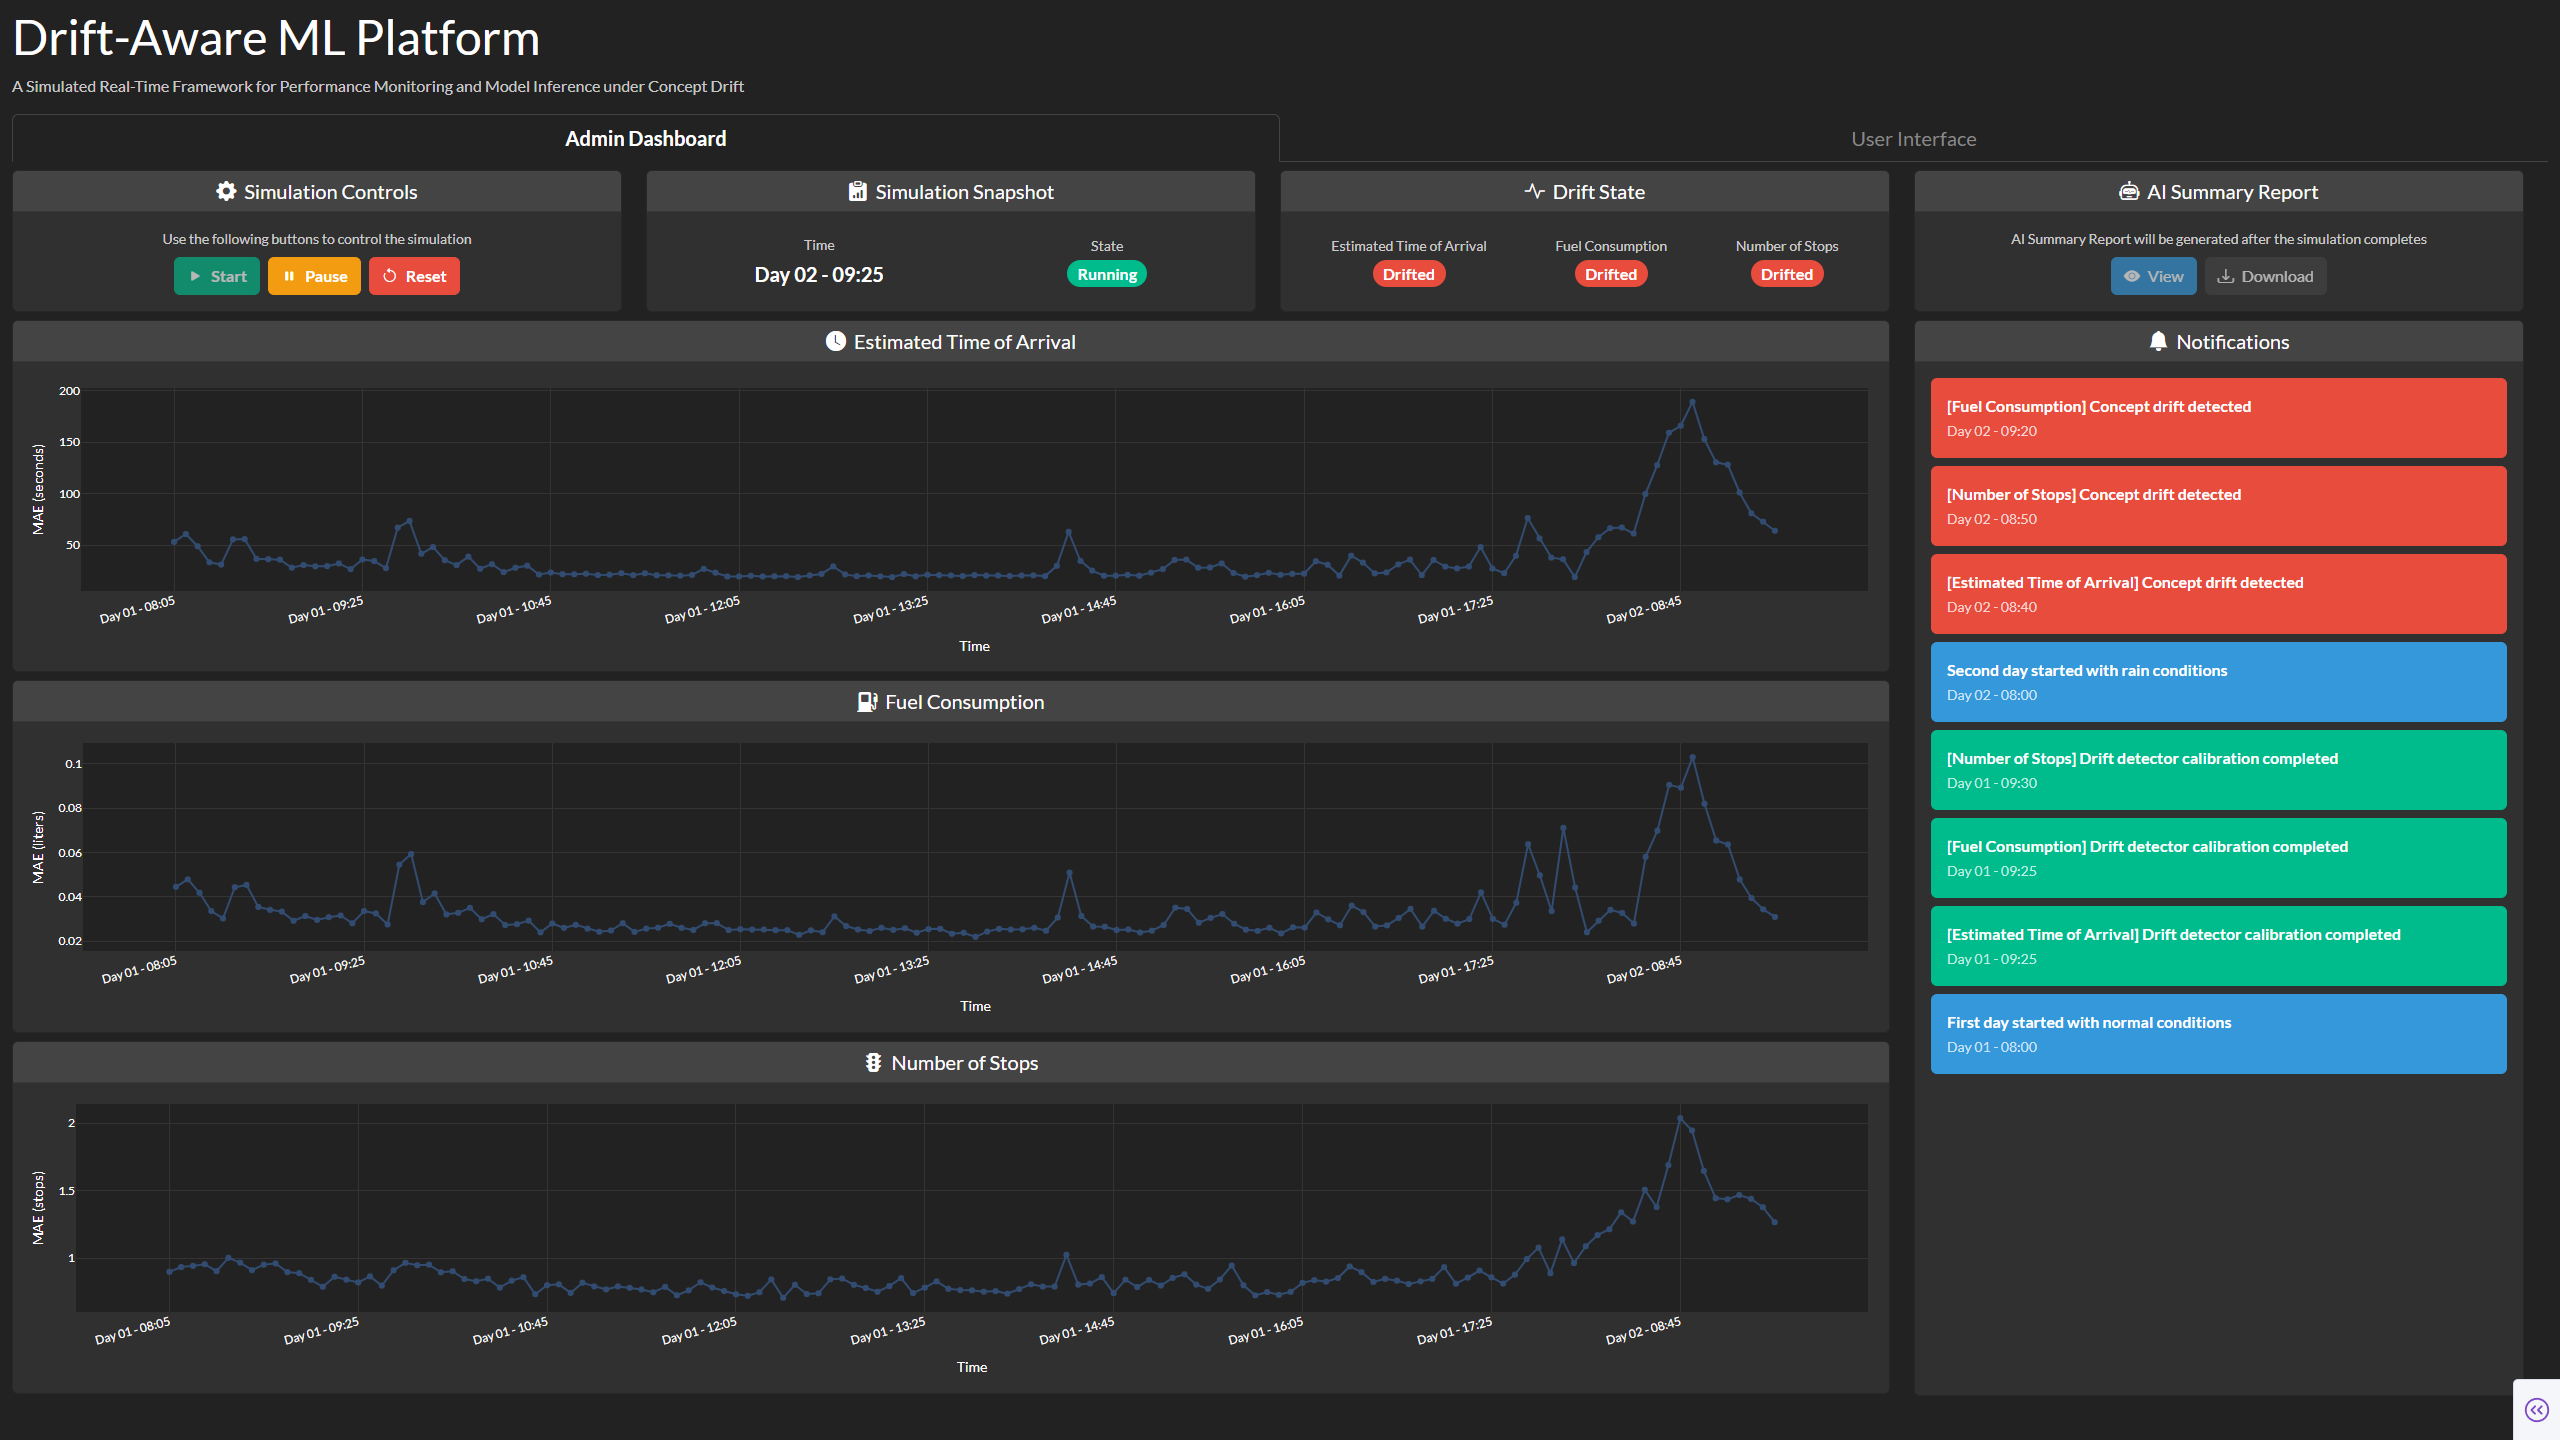
\includegraphics[width=\textwidth]{figures/dashboard-drifted.png}
    \caption{Admin dashboard --- \emph{Drifted}. Rain conditions active, ETA/Fuel/Stops flagged as drifted and errors elevated.}
    \label{fig:dashboard-drifted}
\end{figure}

\clearpage

\begin{figure}[p]
    \centering
    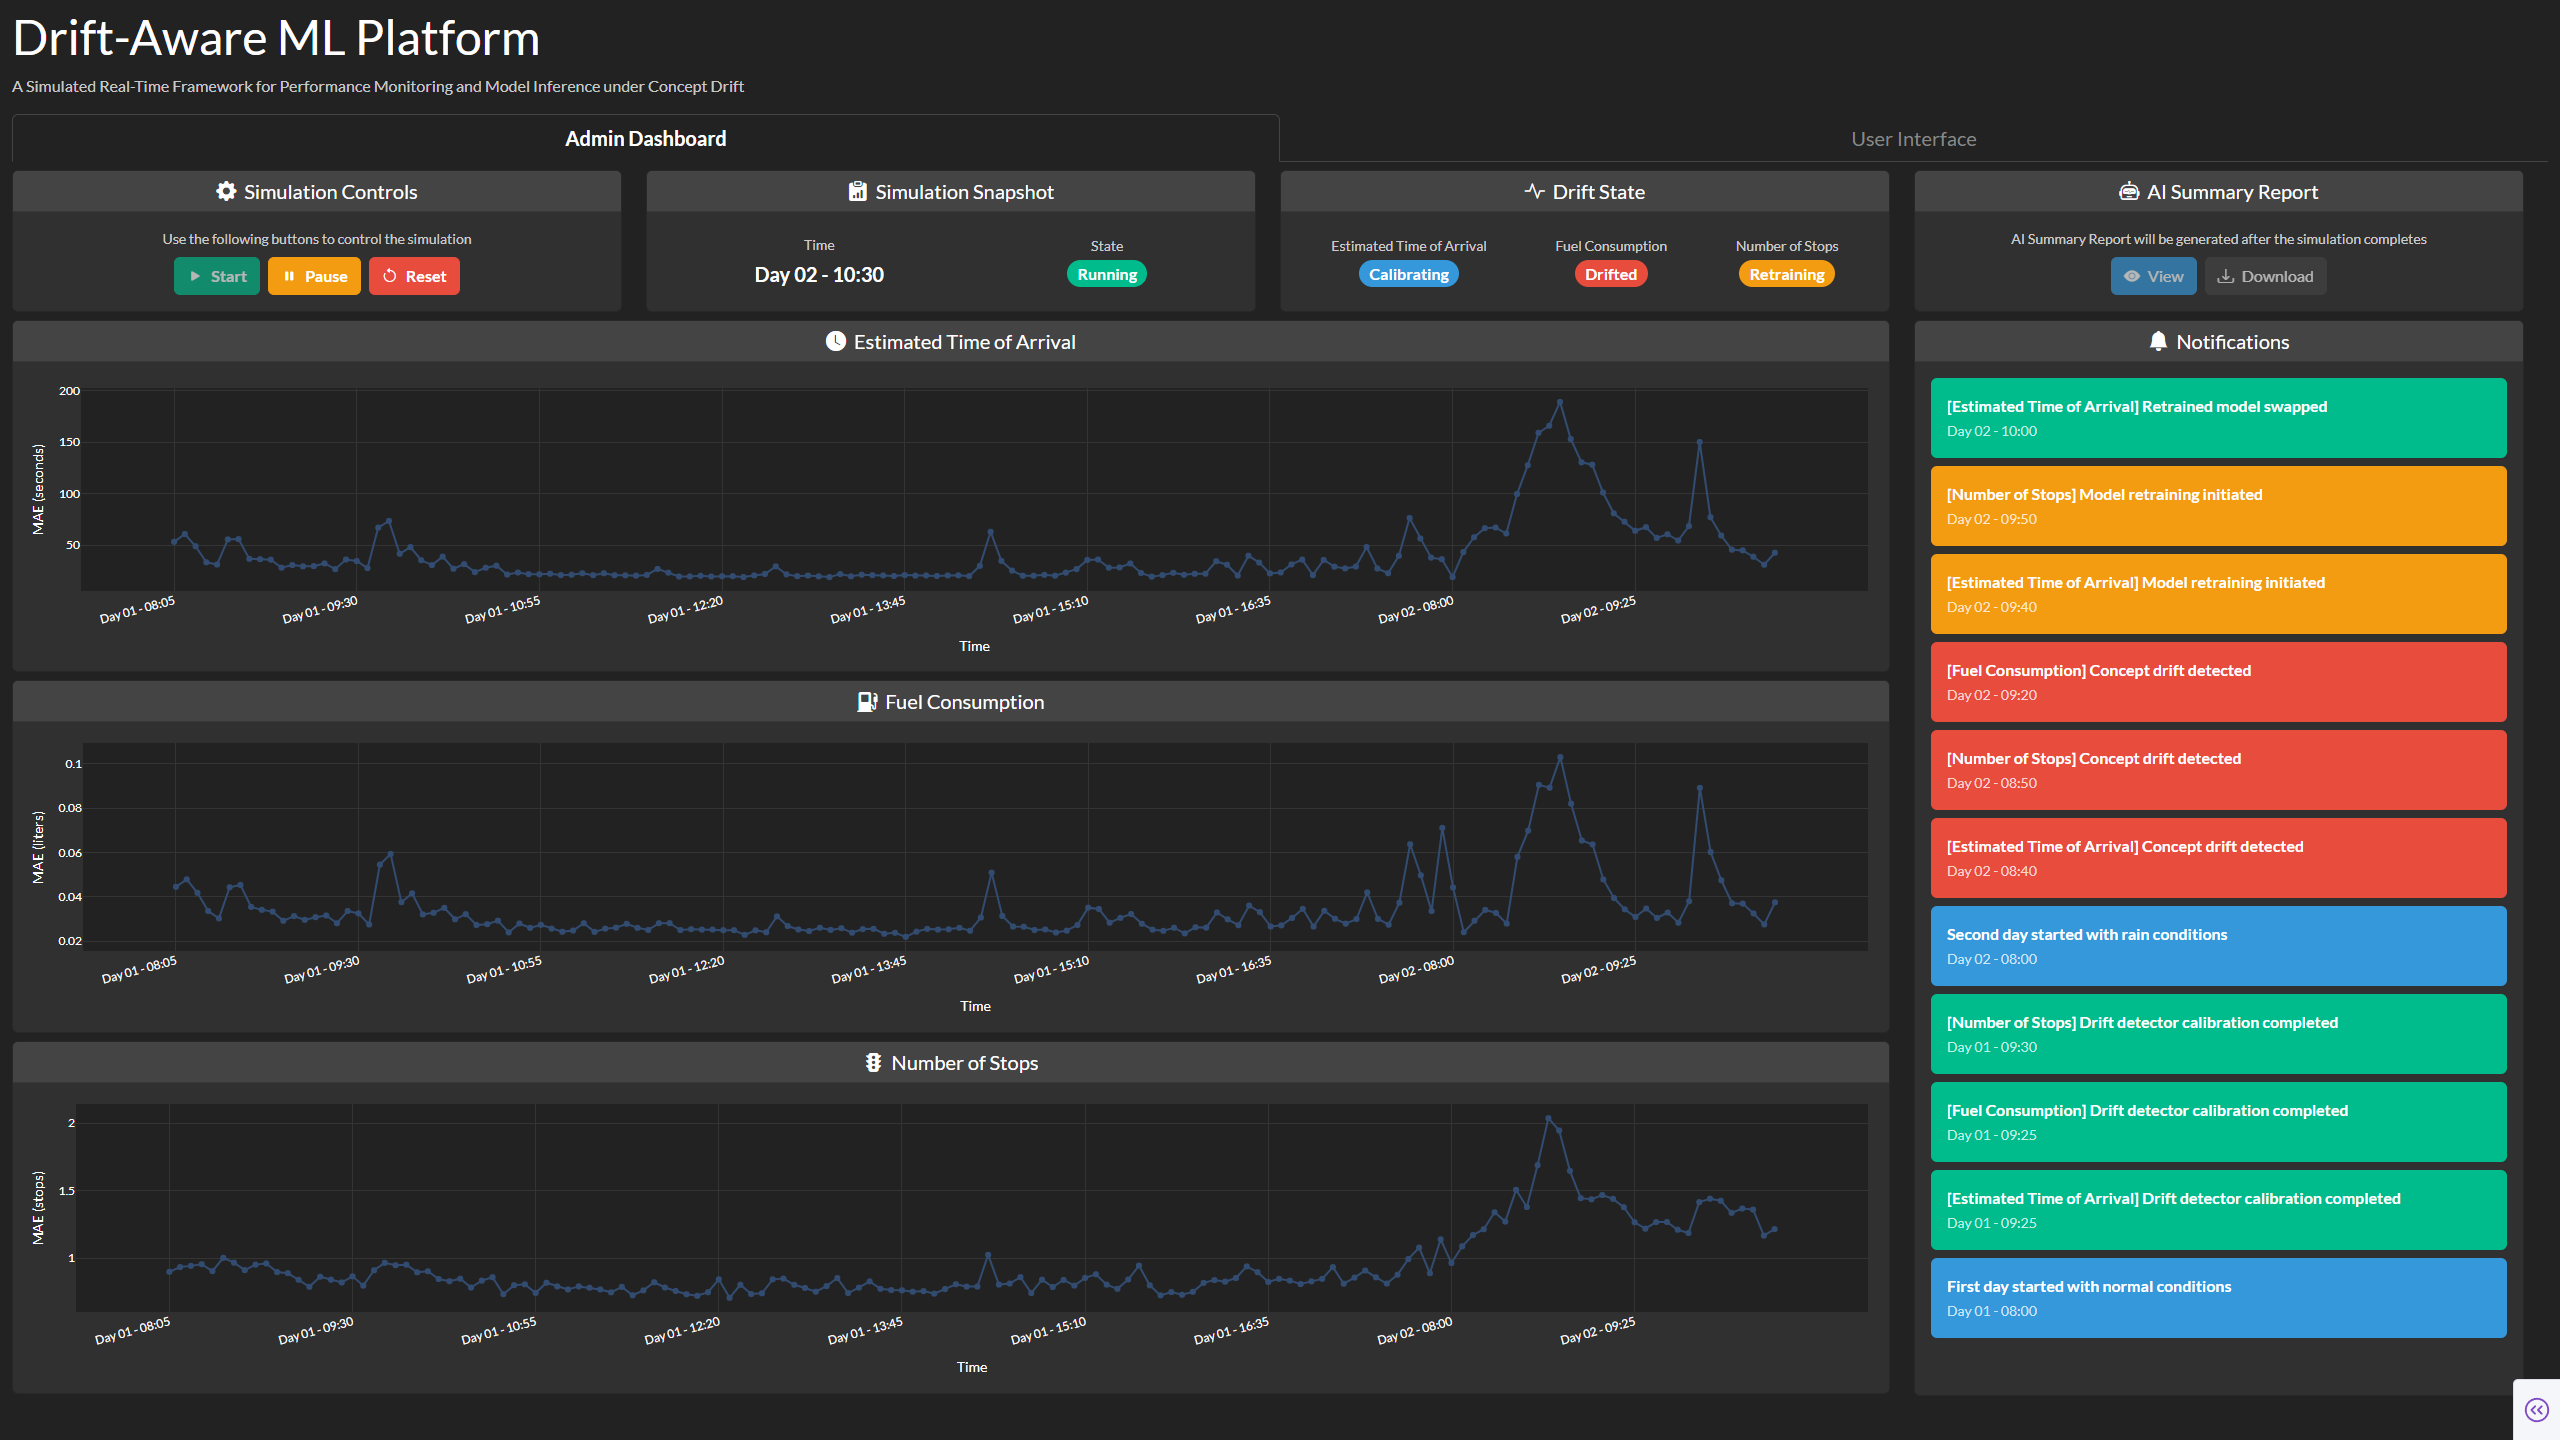
\includegraphics[width=\textwidth]{figures/dashboard-retraining.png}
    \caption{Admin dashboard --- \emph{Retraining}. ETA retrained and swapped, Stops currently retraining, Fuel has not started retraining yet.}
    \label{fig:dashboard-retraining}
\end{figure}

\begin{figure}[p]
    \centering
    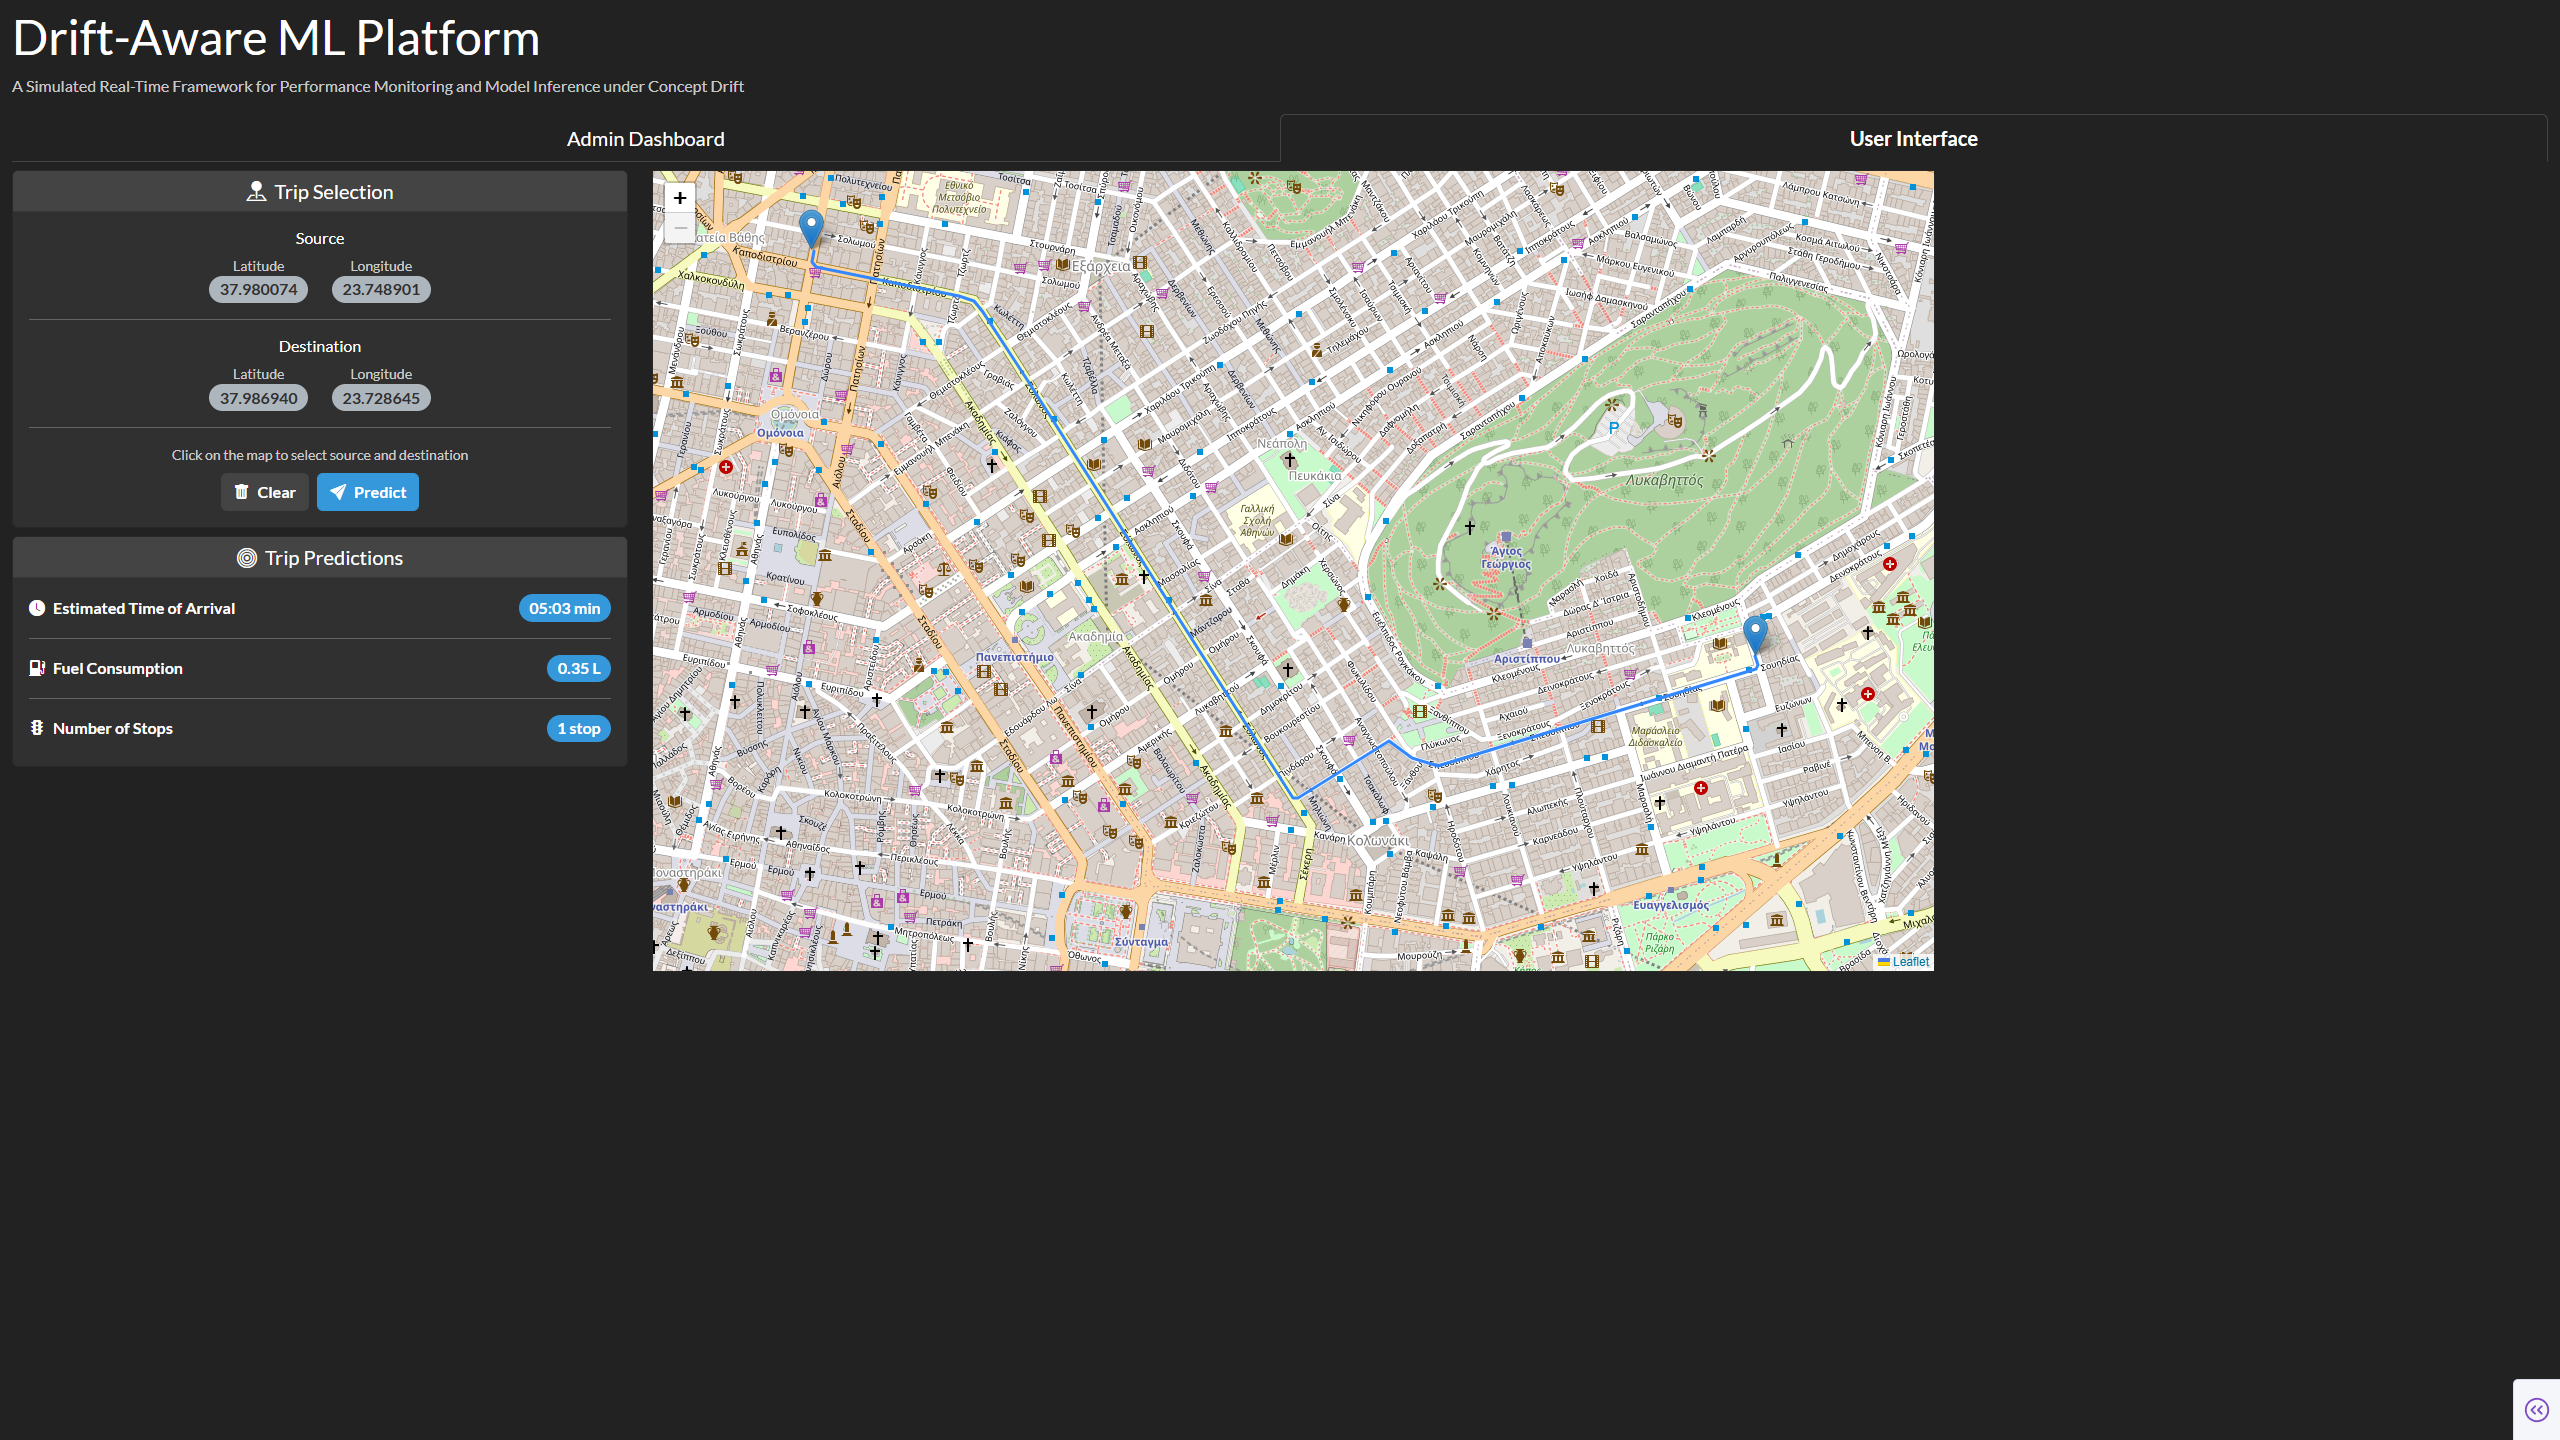
\includegraphics[width=\textwidth]{figures/ui-retraining.png}
    \caption{User interface --- \emph{Retraining}. Same route now reflects rain for ETA only: \texttt{05:03 min}, \texttt{0.35 L}, \texttt{1 stop}.}
    \label{fig:ui-retraining}
\end{figure}

\clearpage

\begin{figure}[p]
    \centering
    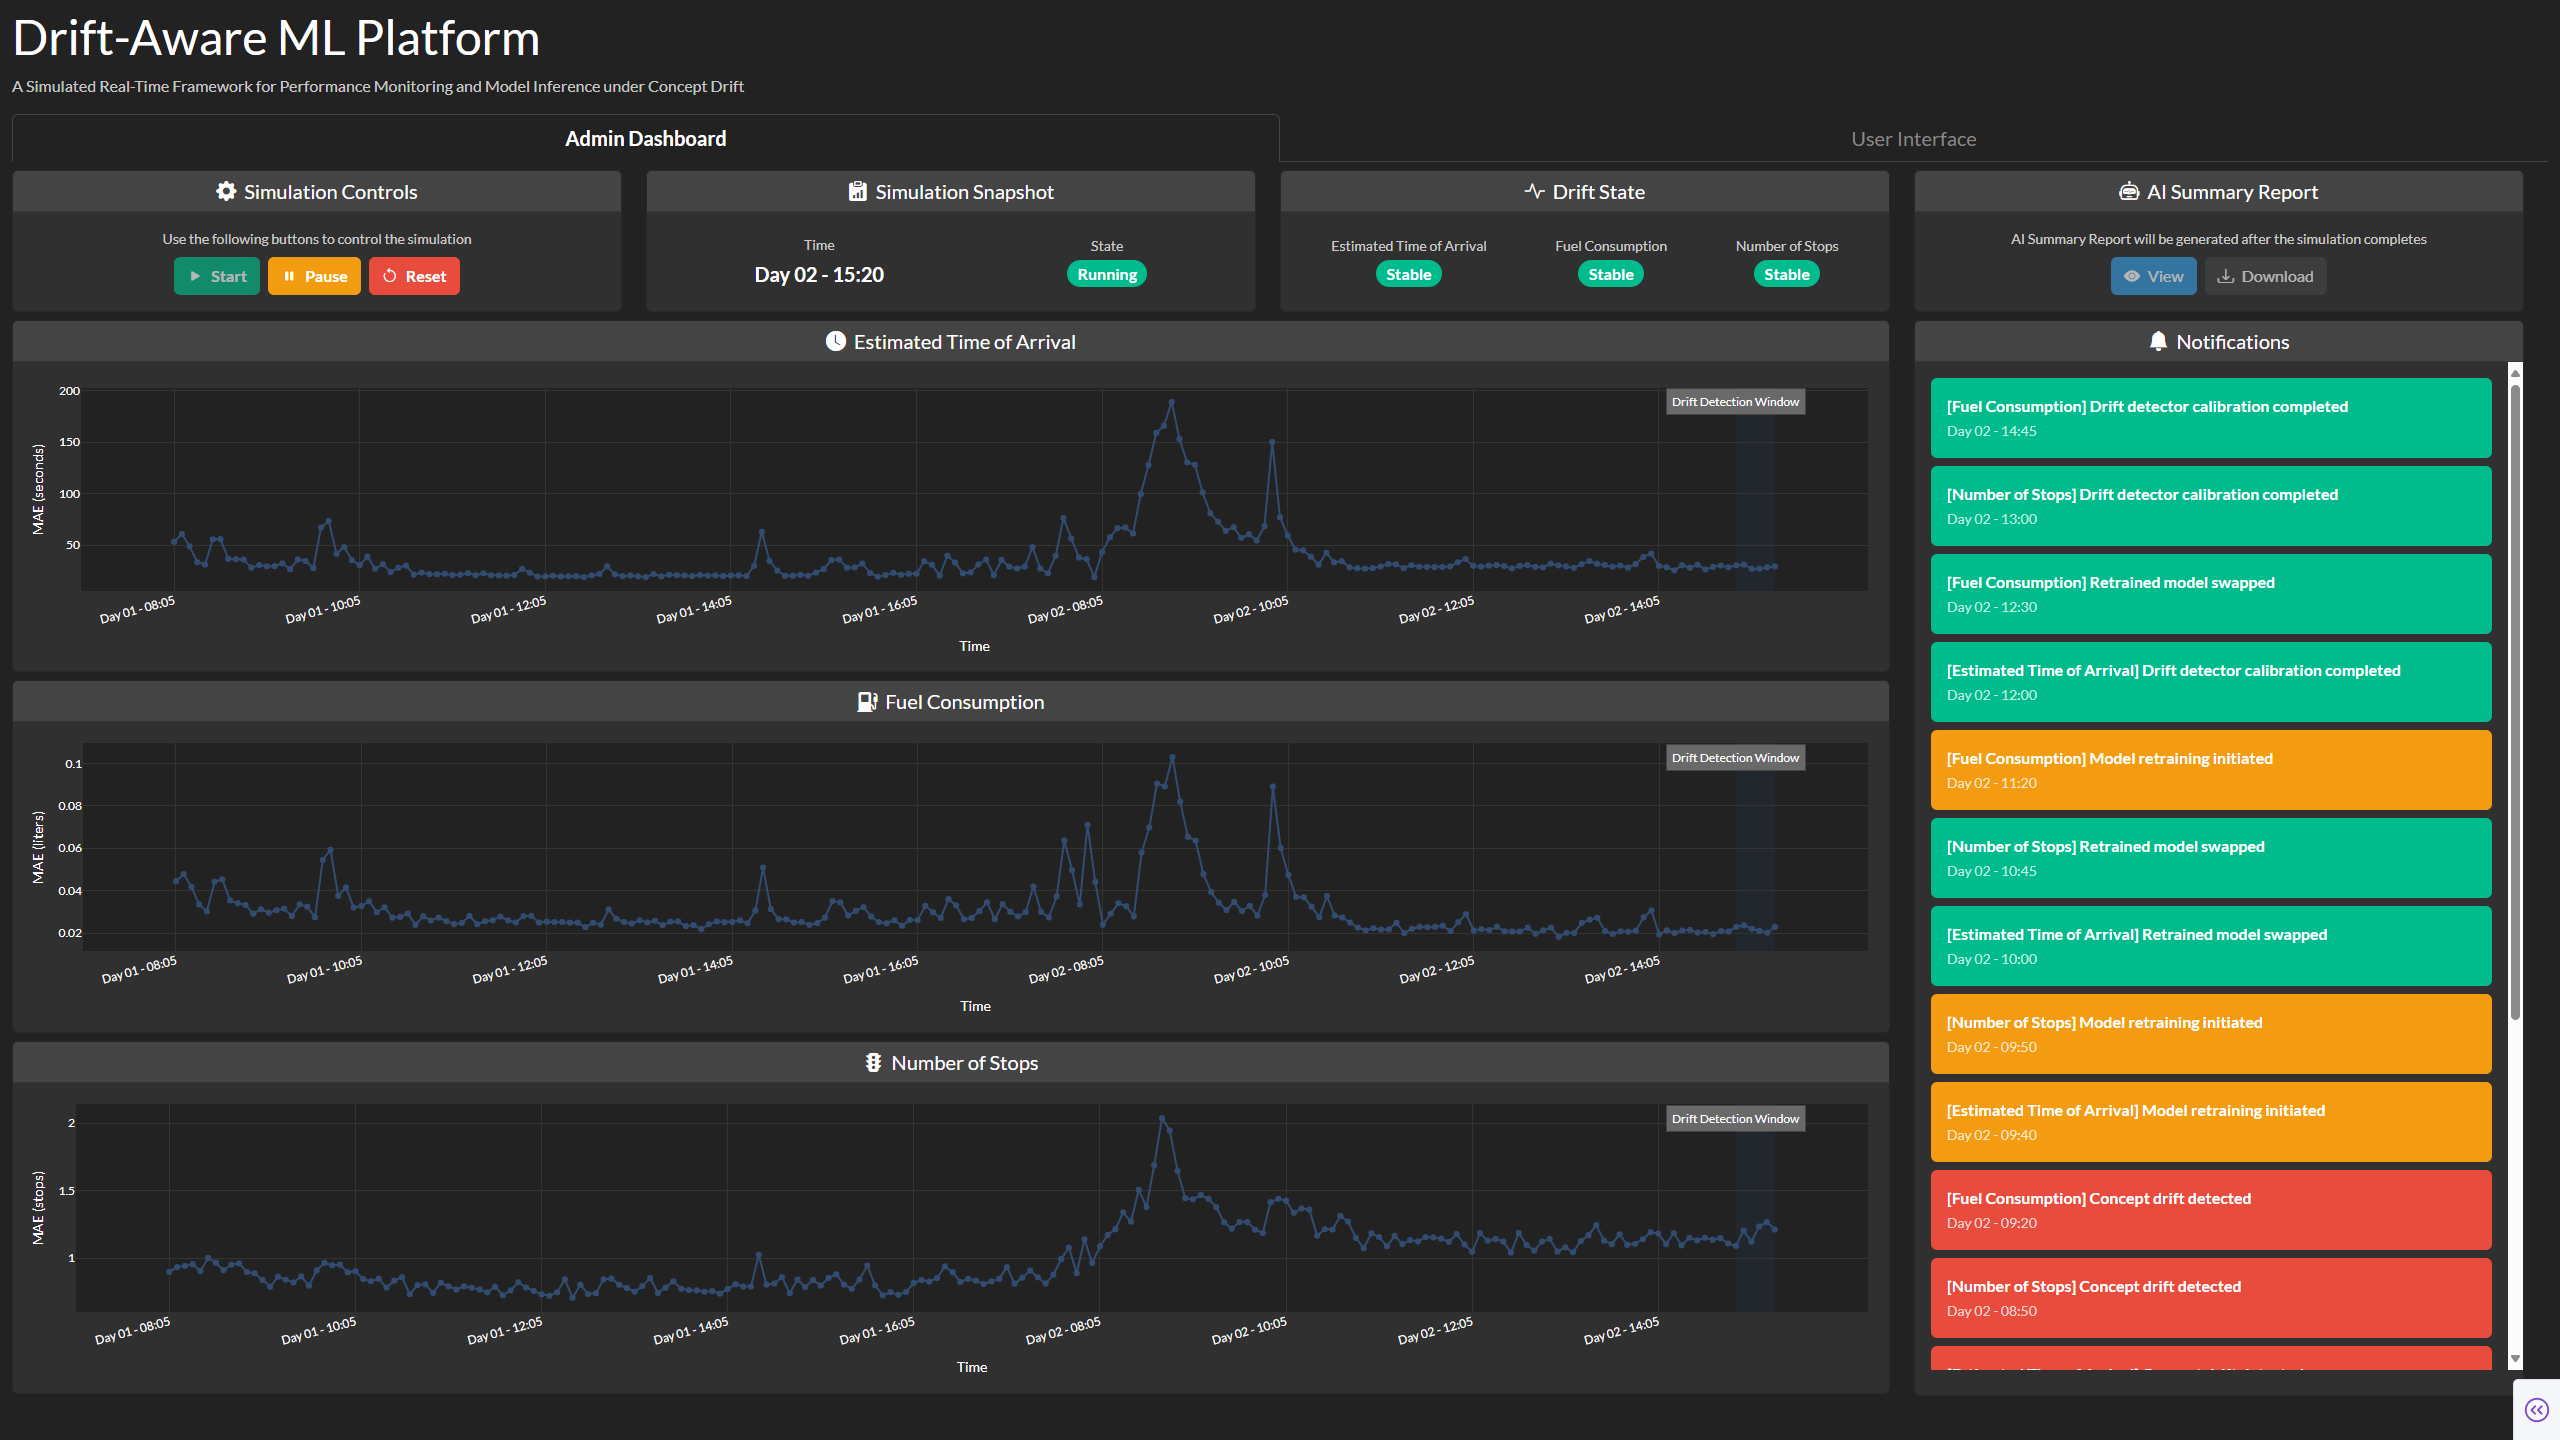
\includegraphics[width=\textwidth]{figures/dashboard-retrained.png}
    \caption{Admin dashboard --- \emph{Retrained}. All three tasks adapted and calibrated, system back to stable.}
    \label{fig:dashboard-retrained}
\end{figure}

\begin{figure}[p]
    \centering
    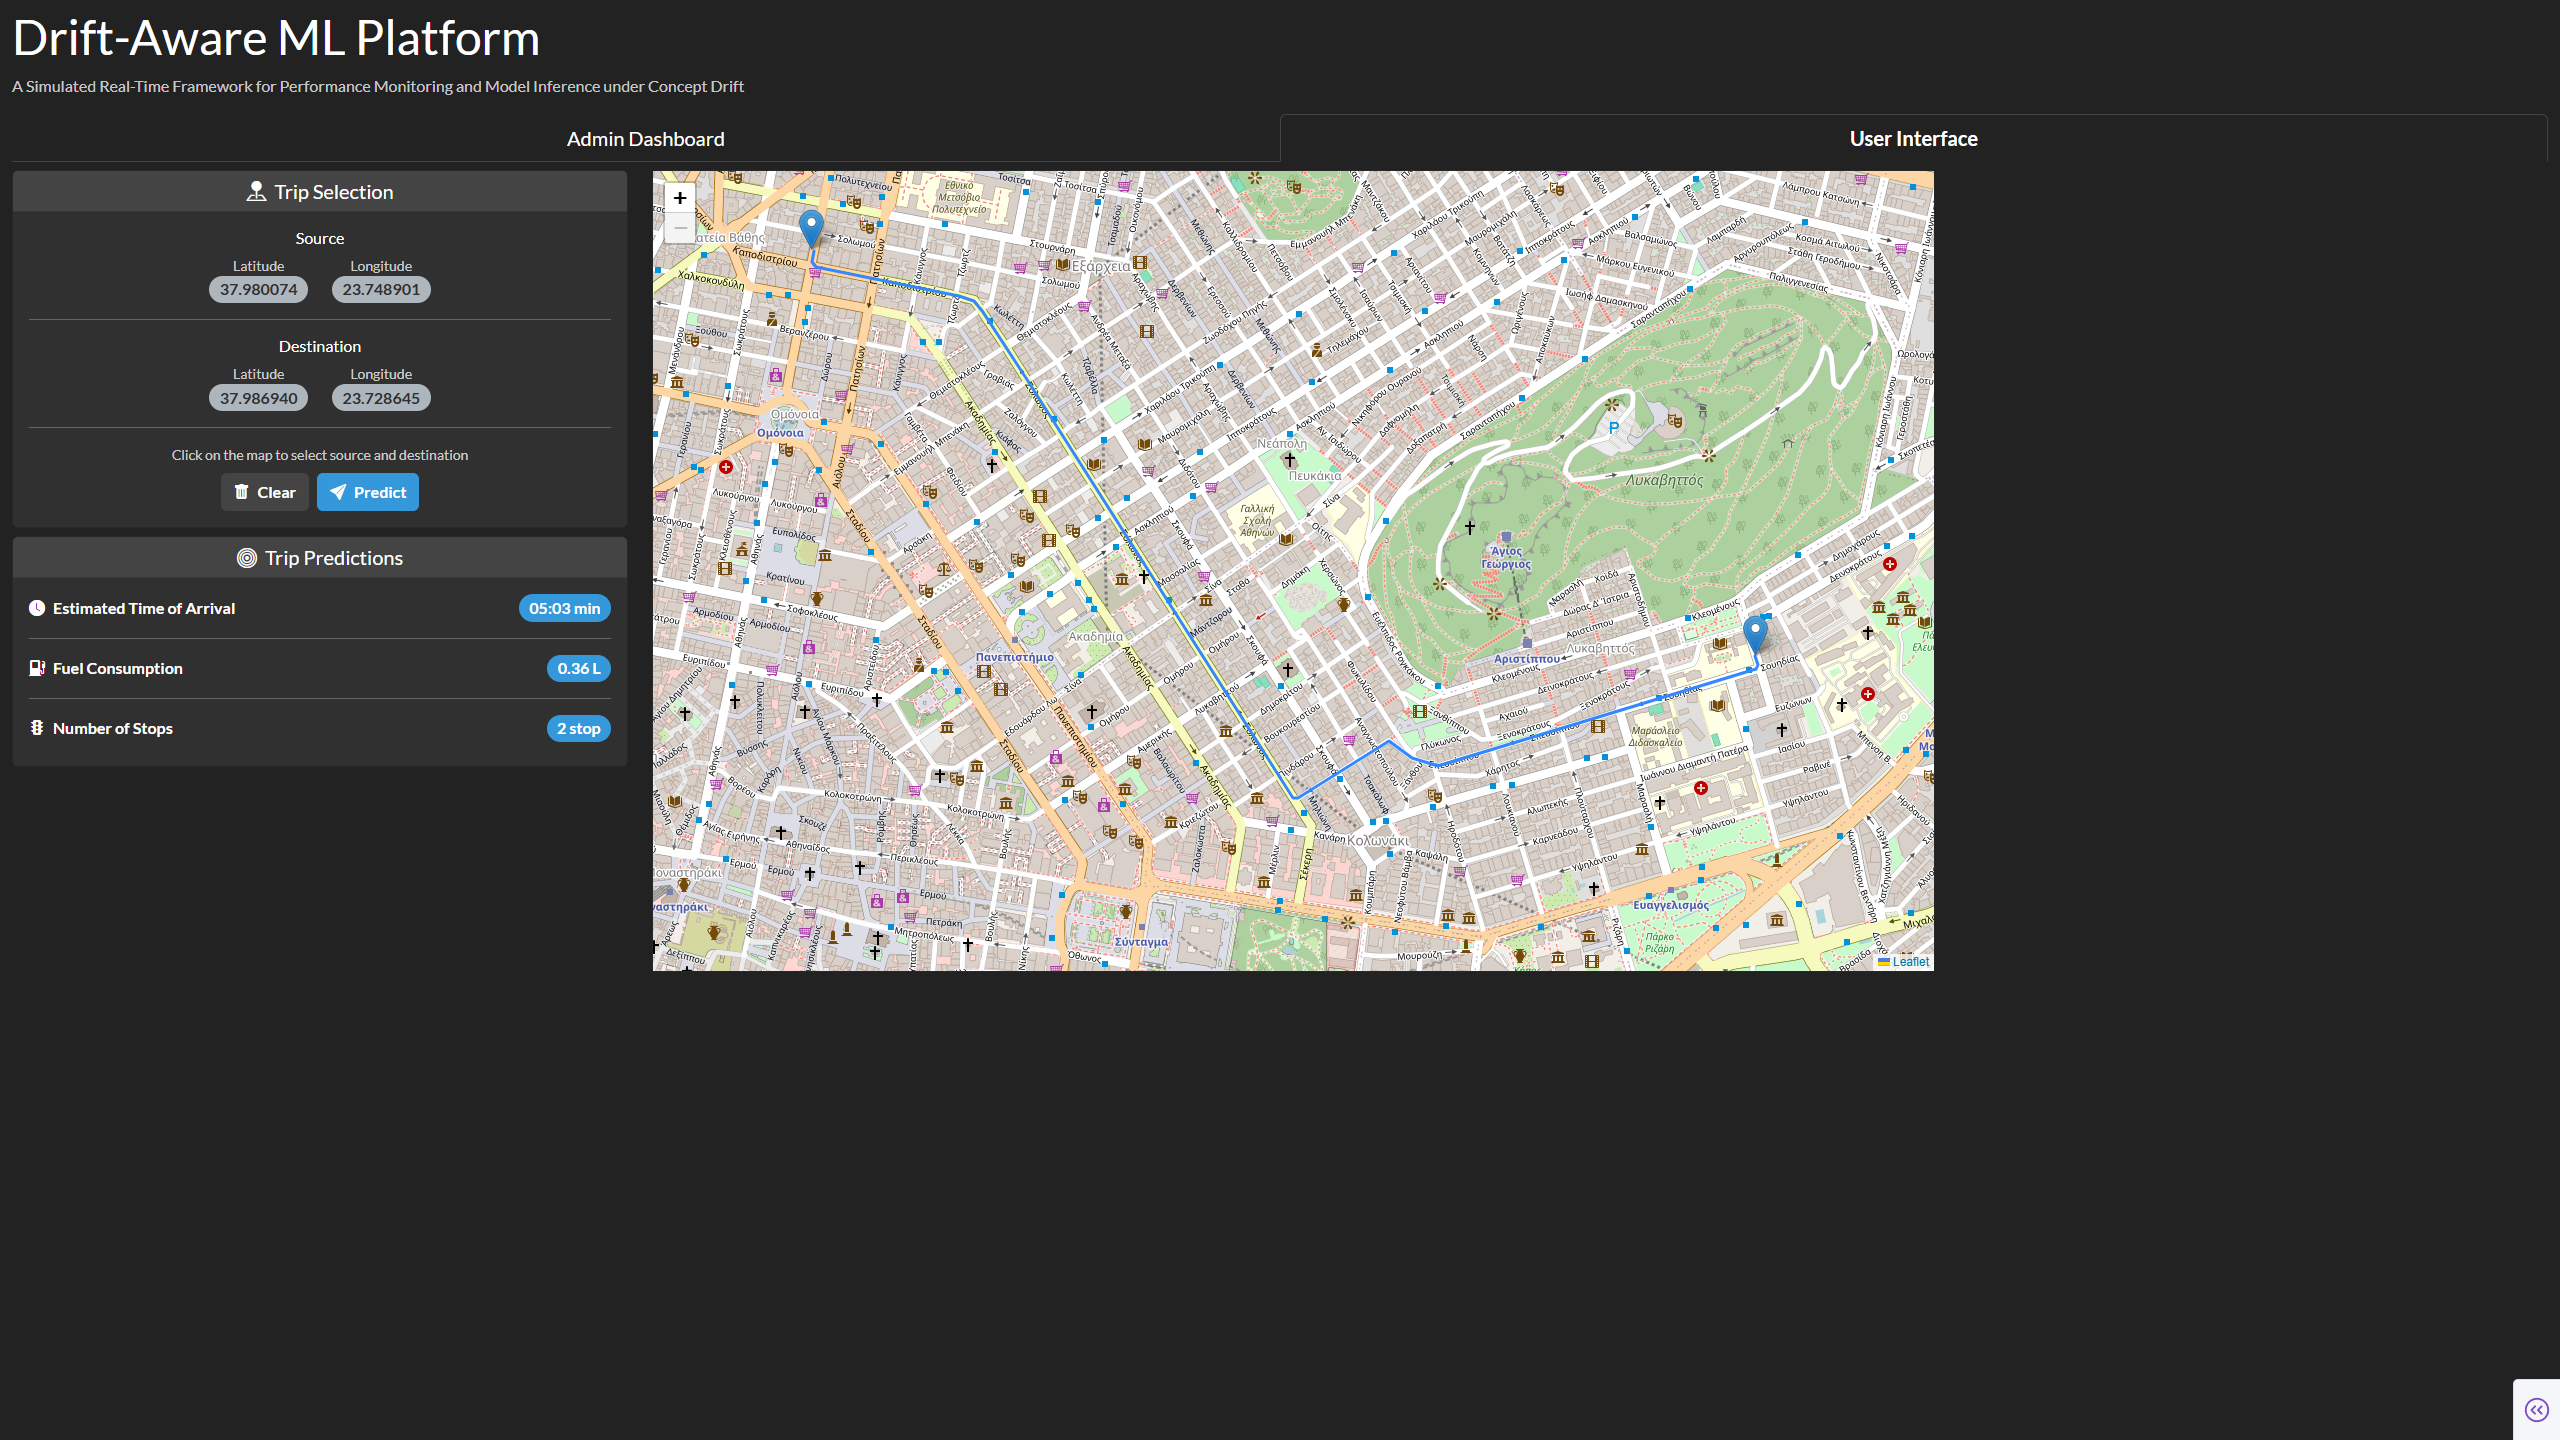
\includegraphics[width=\textwidth]{figures/ui-retrained.png}
    \caption{User interface --- \emph{Retrained}. Same route after full adaptation: \texttt{05:03 min}, \texttt{0.36 L}, \texttt{2 stop}.}
    \label{fig:ui-retrained}
\end{figure}

\clearpage

\begin{figure}[p]
    \centering
    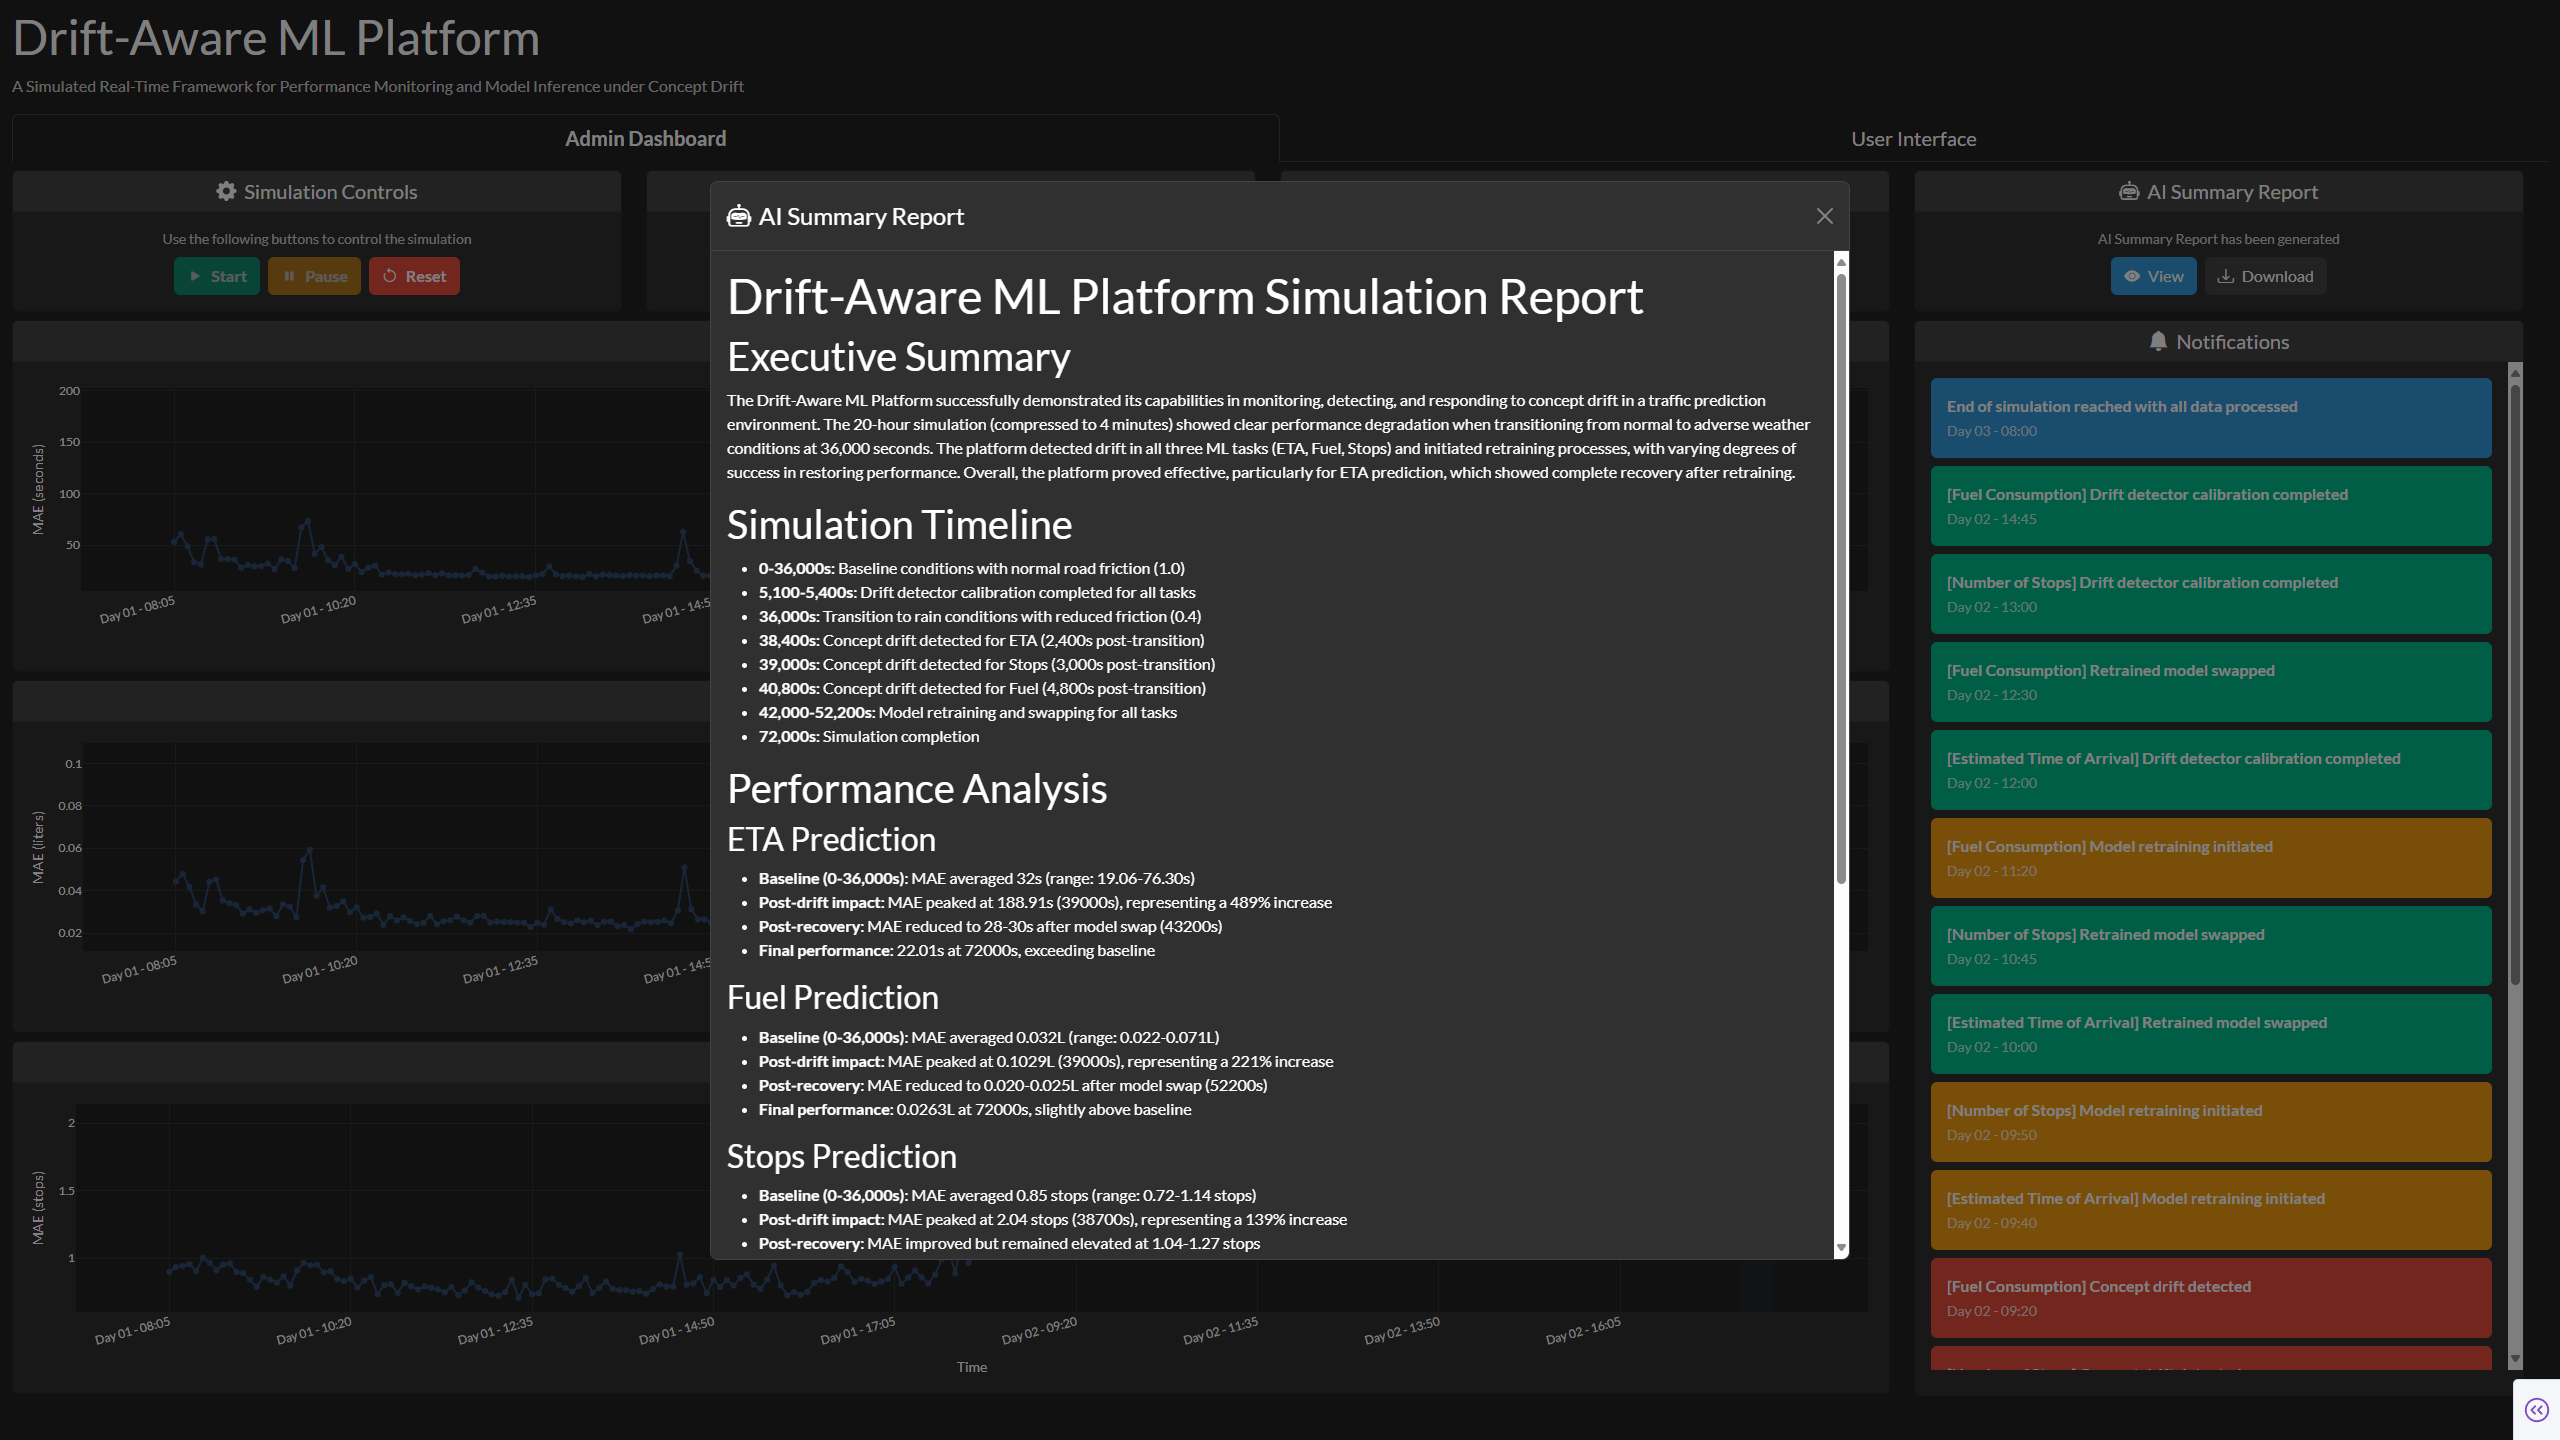
\includegraphics[width=\textwidth]{figures/dashboard-report.png}
    \caption{AI summary report shown in Admin Dashboard after simulation completion.}
    \label{fig:dashboard-report}
\end{figure}
